\documentclass[oneside]{report}

\usepackage{fancyhdr}
\usepackage[utf8]{inputenc}
\usepackage[T1]{fontenc}
\usepackage{titlesec}

\usepackage{geometry}
\geometry{margin=1.4in}
\newcommand{\timelineFormat}{\hspace{-2.3pt}$\bullet$ \hspace{5pt}}
\setlength\parindent{0pt}
\setlength{\parskip}{0.4cm}

\usepackage{pdfpages}
\usepackage{graphics}
\usepackage{graphicx}
\usepackage{float}
\usepackage[english]{babel}
\usepackage{xspace}
\usepackage{lipsum}

% ¤¤ Navngivning ¤¤ %
\addto\captionsdanish{
    \renewcommand\contentsname{Table of Contents}
}

%Initializing packages
\usepackage{adjustbox}
\usepackage{textcomp}
\usepackage{booktabs}
\usepackage{csquotes}
\usepackage{mathtools}
\usepackage[normalem]{ulem}
\useunder{\uline}{\ul}{}

\usepackage{eurosym}
\usepackage{forest}
\usepackage{lscape}
\usetikzlibrary{arrows.meta}
\usepackage{tabularx}
\usepackage{float}
\usepackage{amsmath}
\usepackage{tikz-qtree}
\usepackage{multicol}
\usepackage[bottom]{footmisc}
\renewcommand{\baselinestretch}{1.2}
\usepackage{amsthm}

\theoremstyle{definition}
\newtheorem{definition}{Definition}[section]
\theoremstyle{remark}
\newtheorem*{remark}{Remark}
\usepackage[toc,page]{appendix}
\usepackage{array}
\usepackage[nottoc,notlot,notlof]{tocbibind}
\usepackage{enumitem}
\usepackage{acronym}

% Ekstra pakker
\usepackage{tikz}
\usepackage{placeins}
\usepackage{tikzpagenodes}
\usepackage{xcolor}
\usepackage{graphicx}
\usepackage[utf8]{inputenc}
\usepackage{graphicx}
\usepackage{background} % For AAU wave background
\usepackage{geometry} % For margin adjustments
\usepackage{xcolor}
\usepackage[colorinlistoftodos]{todonotes}
\usepackage{booktabs} % Professional tables
\usepackage{multirow} % Complex table layouts
\usepackage{siunitx} % Proper unit formatting
\usepackage[labelfont=bf]{caption} % Bold captions
\sisetup{per-mode=symbol} % SI unit spacing
\definecolor{aaublue}{RGB}{33,26,82}
\geometry{a4paper} % AAU template assumes A4

\backgroundsetup{contents={}}

\setcounter{tocdepth}{1}

% Tilføjelse af mellemrum mellem "Kapitel" og kapitelnummer i sidehoved med titlesec
\titleformat{\chapter}[display]
  {\normalfont\huge\bfseries}
  {\chaptertitlename\ \thechapter\hspace{1em}} % Tilføjer mellemrum mellem "Kapitel" og kapitelnummer
  {10pt}
  {\Huge}

\titlespacing*{\chapter}{0pt}{-30pt}{20pt}
\setcounter{tocdepth}{3}  % Inkluderer subsections i indholdfortegnelsen.

\usepackage[numbers]{natbib}

\usepackage{caption}
\usepackage{float}
\usepackage{colortbl}  % Pakken til farver i tabeller

\usepackage{hyperref}      % Gør links klikbare og understøtter URL
\hypersetup{
    colorlinks=true,       % Gør links farvede
    linkcolor=blue,       % Farve for interne links
    citecolor=blue,       % Farve for citations
    urlcolor=blue,        % Farve for URL'er
    hidelinks              % Skjuler bokse omkring links
}

\pagestyle{fancy}
\fancyhf{}
\fancyhead[L]{\nouppercase{\leftmark}} 
\fancyfoot[C]{\thepage} 
\renewcommand{\chaptermark}[1]{\markboth{Kapitel \thechapter\hspace{1em}#1}{}}

\begin{document}

\titleformat{\chapter}[display]
    {\bfseries\Huge}{\Large\filleft\MakeUppercase\thechapter}
    {0.5ex}
    {\titlerule}
    [\vspace{1ex}\titlerule]
    \titlespacing*{\chapter}{0pt}{-50pt}{32pt}

\pagenumbering{roman}

\pdfbookmark[0]{Front page}{label:frontpage}%
\begin{titlepage}
\vspace*{\fill}
    \backgroundsetup{
    scale=1.1,
    angle=0,
    opacity=1.0,  %% adjust
    contents={
\includegraphics[width=\paperwidth,height=\paperheight]{7. Figures/AAU baggrund.pdf}}
    }
  \addtolength{\hoffset}{0.5\evensidemargin-0.5\oddsidemargin} %set equal margins on the frontpage - remove this line if you want default margins
  \noindent%
  {\color{white}\fboxsep0pt\colorbox{aaublue}{\begin{tabular}{@{}p{\textwidth}@{}}
    \begin{center}
    \Huge{\textbf{
      SCAN% insert your title here
    }}
    \end{center}
    \begin{center}
      \Large{
        Self-Controlled Aerial Navigation% insert your subtitle here
      }
    \end{center}
    \vspace{0.2cm}
   \begin{center}
    {\Large
      Adam Kuzniewski, \linebreak Emil S. Doganci, \linebreak Mathias M. Larsen% insert names separated by comma
    }\\
    \vspace{0.2cm}
    {\large
      cs-25-sw-6-04% insert name of study, group number, year-month
    }
   \end{center}
   \vspace{0.2cm}
%% Comment this section in if you are doing Bachelor or Master Project   
   \begin{center}
    {\Large
      Bachelor's Project
      %Bachelor Project
    }
   \end{center}
  \end{tabular}}}
  \vfill
  \begin{center}
    
\includegraphics[width=0.2\paperwidth]{7. Figures/AAU logo cirkel.pdf}
    % comment this line in for English version
    %\includegraphics[width=0.2\paperwidth]{Graphics/aau_logo_circle_da} %comment this line in for Danish version
  \end{center}
\end{titlepage}
\clearpage

\thispagestyle{empty}
{\small
\strut\vfill % push the content to the bottom of the page
\centering
\noindent Copyright \copyright{} Aalborg Universitet 2025\par
\vspace{0.2cm}
}
\clearpage


\begin{minipage}[t]{0.42\textwidth}
\vspace{-25pt}

\includegraphics[height=3.7cm]{7. Figures/AAU logo stor dansk.png}
\end{minipage}
\hfill
\begin{minipage}[t]{0.42\textwidth}
{\raggedleft {\small 
\textbf{Software}\\		
Institut for Datalogi\\
Selma Lagerløfs Vej 300\\
9220 Aalborg Øst\\
https://www.dat.aau.dk/\\
}}
\end{minipage}

\vspace*{1cm}

\begin{minipage}[t]{0.42\textwidth}
\textbf{Title:} \\[5pt] 
Self-Controlled Aerial Navigation \vspace*{0.25cm} \\

\textbf{Project Period:} \\[5pt]
03/02/2025 - 28/05/2025 \vspace*{0.25cm} \\

\textbf{Project Group:} \\[5pt]
cs-25-sw-6-04 \vspace*{0.25cm} \\
\\
\textbf{Participant(s):} \\[5pt]
Mathias Mosgaard Larsen \vspace*{0.25cm} \\
Emil Suphi Doganci \vspace*{0.25cm} \\
Adam Kuzniewski \vspace*{0.25cm} \\
\\
\textbf{Supervisor(s):} \\[5pt]
Laurits Brøcker \vspace*{0.25cm} \\
\\
\textbf{Pages:} ANTAL SIDETAL\\

\end{minipage}
\hfill
\begin{minipage}[t]{0.483\textwidth}
\textbf{Abstract}:\\[5pt]
\fbox{\parbox{7cm}{\bigskipAbstract\bigskip}}
\end{minipage}

\vfill
{\footnotesize\itshape }
\chapter*{Preface}
    

\newpage
            
\thispagestyle{empty}
\indent\vspace{80pt}
\begin{minipage}{0.5\textwidth}
    \hrule % Linje
    \vspace{5pt}
    \centering
    {Mathias Mosgaard Larsen\\
    \footnotesize mmla22@student.aau.dk}
\end{minipage}
\begin{minipage}{0.5\textwidth}
    \hrule % Linje
    \vspace{5pt}
    \centering
    {Emil Suphi Doganci\\
    \footnotesize edogan22@student.aau.dk}
\end{minipage}

\vspace{100pt}

\begin{minipage}[b]{0.5\textwidth}
    \hrule % Linje
    \vspace{5pt}
    \centering
    {Adam Kuzniewski\\
    \footnotesize akuzni22@student.aau.dk}
\end{minipage}

\newpage

\tableofcontents
\clearpage

\pagenumbering{arabic}

\chapter{Introduction}

Unmanned Aerial Vehicles (UAVs), or drones, are increasingly being used for aerial surveying and mapping tasks. These drones are typically equipped with cameras capable of capturing high-resolution images of designated areas. The effectiveness of drone-based surveying depends on the flight path used during operation. An optimized flight path covers the entire target area with minimal overlap between the captured images, reducing flight distance and operational time \cite{MathworksUAV}.

Coverage Path Planning (CPP) refers to algorithms designed to compute drone flight paths that ensure full area coverage while minimizing redundant image capture. Commercial drone platforms often use simple predefined patterns, such as lawnmower patterns (boustrophedonic), resulting in significant overlap between images. Research indicates that overlaps exceeding the 75\% front-lap and the 75\% side-lap provide limited additional accuracy but substantially increase the duration of the flight and the workload of data processing \cite{AerotasOverlap}.

Effective CPP algorithms must consider several parameters, including camera field of view (FOV), drone altitude, and ground resolution requirements. The camera FOV determines the ground area captured per image, while altitude directly influences the ground sample distance (GSD), defining image resolution \cite{UAVCoveragePDF}. Incorrect selection or calculation of these parameters can result in either excessive overlap or incomplete coverage \cite{OptimizationUAV}.

The Self-Controlled Aerial Navigation (SCAN) project aims to develop a system capable of generating optimized drone flight paths based on user-defined survey areas. The goal is to minimize redundant coverage and total flight distance while ensuring complete area coverage with adequate image resolution. Specifically, the project focuses on optimizing paths to facilitate human detection from drone imagery, making the solution applicable for Search and Rescue (SAR) scenarios.

Existing CPP approaches include exact cellular decomposition methods \cite{UAVCoveragePDF}, wavefront algorithms, and traveling salesman problem (TSP)-based solutions \cite{SmoothCoverage}. However, these methods do not specifically address practical constraints such as camera FOV optimization or human detection requirements encountered in SAR operations. For instance, SAR missions require capturing images at resolutions suitable for reliable human identification \cite{NorwegianPolice}.

The SCAN system combines these algorithmic considerations with practical implementation by allowing users to select survey areas on an interactive map interface. The system then autonomously generates an optimized flight plan for the drone to execute. Additionally, SCAN integrates object detection capabilities to identify humans within surveyed areas and map their positions onto the user interface.

\section{Initial problem statement}

Drones are commonly employed for aerial surveying tasks in various fields including agriculture, construction, environmental monitoring, and search and rescue operations. Current commercial drone solutions typically utilize basic predefined flight patterns with fixed overlap settings. These standard approaches often result in redundant data collection, increased flight time, and higher processing demands without proportional improvements in survey accuracy \cite{AerotasOverlap}.

The SCAN project addresses this issue by developing optimized path planning algorithms specifically designed for drone-based aerial surveying tasks. The primary objective is to create a flight path that minimizes total travel distance while ensuring full coverage of a selected area at sufficient image resolution for reliable human detection.

Several factors must be considered when developing optimized flight paths:

First, the drone's camera field of view directly affects ground coverage per image. Ignoring this parameter can lead to unnecessary overlap or gaps in coverage \cite{UAVCoveragePDF}. Accurate calculations involving camera FOV and drone altitude are required to determine optimal spacing between adjacent flight lines.

Second, minimizing total travel distance while maintaining complete coverage presents an optimization problem similar to known computational geometry problems such as the traveling salesman problem (TSP). Existing solutions such as grid-based decomposition or wavefront algorithms have limitations when applied practically to aerial surveying tasks involving irregularly shaped areas or obstacles \cite{SmoothCoverage}.

Third, there is a trade-off between altitude selection and image quality. Higher altitudes increase coverage per image but reduce spatial resolution required for accurate human detection \cite{OptimizationUAV}. For example, guidelines from Norwegian Police SAR operations recommend specific altitudes (approximately 100 meters above ground level) combined with defined camera angles to achieve suitable resolution for human identification tasks \cite{NorwegianPolice}.

To effectively address these challenges, the following research questions are defined:

\begin{itemize}
    \item Which algorithms can generate optimized drone flight paths that minimize total travel distance while ensuring complete area coverage?
    \item How can optimal drone altitude and flight line spacing be calculated based on camera field of view to achieve required image resolution?
    \item How can object detection methods be integrated into aerial surveying workflows for automatic identification and mapping of humans within surveyed regions?
    \item What methods can be used to evaluate algorithm performance under realistic operational conditions?
\end{itemize}

The SCAN project focuses specifically on addressing these research questions through algorithm development, practical experimentation, and validation tests aimed at demonstrating applicability in scenarios such as search and rescue operations.

\chapter{Problem Analysis}

\section{System Integration Challenges in Maritime Search and Rescue}

Maritime search and rescue (SAR) operations typically require the use of multiple separate tools for mission planning, drone control, data collection, and analysis~\cite{connectivity_challenges_2024, uav_holistic_2024}. While platforms such as PX4 and ArduPilot provide automated grid-based path planning features-allowing users to define search areas and generate systematic flight paths for coverage~\cite{ardupilot_grid_2023, px4_mission_2024}-these solutions primarily address the planning and navigation stages. Operators must still manually transfer data between mission planning software, flight control interfaces, and post-mission detection or analysis tools.

Although auto-grid and survey functions in tools like Mission Planner and QGroundControl facilitate the creation of efficient coverage paths, there are notable limitations in the context of maritime SAR. First, these workflows do not natively integrate real-time or automated person detection; image analysis is typically performed after the mission using separate applications, which can delay rescue efforts. Second, standard grid-based planning tools are designed for general aerial surveys and may not account for maritime-specific challenges such as wave motion, water surface reflections, or the need for altitude adjustments to ensure reliable detection of small objects in water~\cite{SARSurvey2024}. Third, the lack of a unified workflow means that operators are required to have technical knowledge of multiple platforms and must coordinate data flow between them, which increases the risk of errors and slows down the response process.

The absence of end-to-end integration-from area definition through flight execution to automated detection and result presentation-remains a gap in current drone-based SAR solutions. This fragmentation is particularly problematic in time-sensitive maritime environments, where rapid transitions from search area definition to actionable detection results are essential for effective rescue operations.


\section{Software Framework Evaluation}
% Analysis of why we chose to work with SDK's over the other options.
The selection of a software framework for the SCAN project involved considering multiple different approaches to drone control, the development process, and the limitations of the project resources. 

\subsection{Available Options}
The project team considered the following approaches:

\begin{itemize}
    \item Building a custom drone
    \item Custom firmware development
    \item Open-source flight control software
    \item Manufacturer-provided SDKs
\end{itemize}

Each option was evaluated on the basis of the project's requirements and constraints.

\subsection{Building a Custom Drone}
The option of building a custom drone from scratch was initially considered. This approach would involve the following.

\begin{itemize}
    \item Selecting and assembling hardware components (frame, motors, flight controller, etc.)
    \item Building a fundamental frame by hand or 3D printed for all the components.
    \item Configuring the flight controller.
    \item Developing custom software for drone control
\end{itemize}

This process would require a high initial cost for components and an unreasonable time investment for assembly and configuration. It would also necessitate some more specialized knowledge in electronics and drone mechanics, which falls outside the project's primary scope and focus on software engineering. 

\subsection{Custom Firmware Development}
Custom firmware development involves writing low-level code to directly control drone hardware. This approach is as follows.

\begin{itemize}
    \item More flexibility in terms of drone behavior
    \item Full control over all aspects of the drone's operation
\end{itemize}

The primary disadvantage of firmware development for the project team is the lack of experience developing software at this level, which consequentially would narrow down the scope even further due to the resource limitations, specifically in terms of time. The majority of the time spent on the project would be on understanding the development of the firmware and low-level interactions with the hardware.

\subsection{Open-Source Flight Control Software}
Open-source options such as ArduPilot and PX4 were evaluated. These frameworks offer the following.

\begin{itemize}
    \item Many customization options
    \item Large community support
    \item Compatibility with various drone hardware
\end{itemize}

Similarly, the primary disadvantage of open source flight control systems is the lack of experience in the project team. In addition to having a steep learning curve as suggested by multiple sources\cite{mdpi_px4_survey,oscarliang_ardupilot,bluefalcon_sdk}, there is also more limited official support compared to manufacturer SDKs, which in terms of risk management would be a poor decision to make.

\subsection{Manufacturer-Provided SDKs}

The evaluation of manufacturer-provided SDKs focused on the Parrot Olympe SDK and DJI's SDKs, as these matched the drone platforms supplied by the university for the project. Two main options were considered: the Parrot Olympe SDK and DJI's SDK. The Parrot Olympe SDK, compatible with the Parrot ANAFI drone, offers a Python-based API for flight control, camera operation, and access to telemetry data such as coordinates and temperature~\cite{ParrotSDKDoc}. Parrot also provides several other SDKs, including GroundSDK for mobile application development, AirSDK for onboard programming, Sphinx for simulation, and PDrAW for video streaming.

DJI offers a range of SDKs as well, including the Mobile SDK for Android and iOS, the Windows SDK for web applications, the Onboard SDK for direct integration with flight controllers, and the Payload SDK for external sensor or payload integration~\cite{DJIDocumentation}. These SDKs provide access to flight control, telemetry, camera, gimbal, and obstacle avoidance features.

Key considerations in selecting an SDK included access to telemetry data (such as GPS) and camera functionality for object recognition, as well as the ability to run the SDKs on the team's development machines. A notable limitation was that Parrot Olympe only runs on Ubuntu Linux, and using it on ARM64 (such as Apple Silicon MacBooks) requires containerizing Ubuntu and compiling Parrot Olympe manually, which could introduce compatibility issues for team members using macOS.

\section{Drone Selection Process}
% Analysis of the required hardware for the drone, the different drones we tested etc.
In selecting a drone for an academic project, the team identified several requirements. These included an SDK for remote control, GPS for autonomous flight coordination, and a quality camera for area mapping and image recognition.

Research pointed to Parrot as a good option, with drones featuring fully customizable SDKs meeting all criteria. This discovery was initially met with optimism. However, due to equipment limitations, the project team was first provided with the DJI Mini Pro 3 drone.

The DJI Mini Pro 3 is a high-end drone that appeared to meet project requirements with its features, including a good SDK, premium camera, and GPS. Yet during testing, the team found that the stock controller was locked down, preventing custom programming. This made the DJI Mini Pro 3 unsuitable for the project.

After this setback, the equipment team acquired a Parrot ANAFI drone. This model proved to be an excellent match for the project and satisfied all requirements. The Parrot ANAFI offers flexible control options, allowing operation through either the included controller or by connecting to the drone's system via a smartphone.

A major advantage of the Parrot ANAFI is its compatibility with the "Olympe" SDK from Parrot. This SDK allows custom scripts to run on the drone by connecting from a PC. Testing confirmed that the Parrot ANAFI was indeed the right choice, meeting all project requirements and providing the flexibility to implement the desired search pattern algorithm and other custom functions.

The selection of the Parrot ANAFI represents progress in the project, giving the team the tools needed to develop autonomous flight and area mapping capabilities. This choice enables further advances in academic research, potentially leading to applications in search and rescue or environmental monitoring.

\section{Communication Architecture}
Effective drone operations are critically dependent on reliable communication between the aerial vehicle and ground control systems. Communication architectures for unmanned aerial systems must address fundamental challenges including transmission reliability, bandwidth management, range limitations, and resilience to interference \cite{Sharma2017}. These factors directly impact system capabilities, operational safety, and mission effectiveness, particularly in search and rescue applications where real-time control and data transmission are essential \cite{Erdelj2017}.

\subsection{General Communication Challenges in Drone Systems}

Drone communication systems face unique challenges distinct from traditional networked applications:

\begin{itemize}
    \item \textbf{Three-dimensional mobility}: As drones move through space, connection quality typically varies with distance, orientation, and obstacles \cite{Zeng2016}
    \item \textbf{Bandwidth constraints}: Multiple data streams (control commands, telemetry, and video) must share limited wireless bandwidth \cite{Hayat2016}
    \item \textbf{Safety-critical nature}: Unlike with consumer applications, communication failures can result in physical damage or loss \cite{Koubaa2019}
    \item \textbf{Electromagnetic interference}: Drones operate in varying electromagnetic environments that can impact signal integrity \cite{Fotouhi2019}
    \item \textbf{Regulatory restrictions}: Communication systems must comply with regional frequency regulations and power limitations \cite{Gupta2016}
\end{itemize}

Any drone communication architecture must address these fundamental challenges through appropriate protocols, hardware configurations, and software management strategies.

\subsection{Parrot ANAFI Communication Infrastructure}

For the SCAN project, the selected Parrot ANAFI platform implements a specific communication architecture. According to manufacturer specifications, the ANAFI uses a Wi-Fi-based communication system with the following characteristics:

\begin{itemize}
    \item Creates an on-board Wi-Fi access point (2.4GHz or 5GHz bands) \cite{ParrotANAFISpec}
    \item Utilizes proprietary protocols built on standard TCP/IP and UDP connections \cite{ParrotSDKDoc}
    \item Supports a theoretical range of up to 4 km under optimal conditions \cite{ParrotANAFISpec}
    \item Implements automatic frequency band selection to minimize interference \cite{ParrotSDKDoc}
    \item Employs dynamic signal strength management to maintain connection stability \cite{ParrotSDKArch}
\end{itemize}

The reliance on Wi-Fi technology represents a specific implementation approach to addressing the general communication challenges. While enabling straightforward connectivity and sufficient bandwidth for control and video transmission, Wi-Fi is susceptible to interference in crowded RF environments and has inherent range limitations compared to dedicated long-range communication systems \cite{Yanmaz2018}.

\subsection{Olympe SDK Communication Model}

The Olympe SDK provides an abstraction layer for communicating with the ANAFI drone through a structured API \cite{ParrotOlympeDoc}. This software architecture shapes how applications can interact with the drone's communication systems:

\begin{itemize}
    \item Implements Python-based command structures that are translated into the drone's proprietary protocol
    \item Manages the connection establishment and maintenance automatically
    \item Provides event-driven callbacks for asynchronous status updates and telemetry
    \item Handles media streaming through dedicated protocol handlers
    \item Offers automatic reconnection capabilities during temporary signal loss
\end{itemize}

Through analysis of the SDK documentation \cite{ParrotOlympeDoc}, it can be determined that Olympe uses multiple communication channels with different protocols:

\begin{table}[h]
\centering
\caption{ANAFI Communication Channels}
\label{tab:anafi_channels}
\begin{tabular}{@{}llll@{}}
\toprule
\textbf{Channel} \& \textbf{Protocol} \& \textbf{Purpose} \& \textbf{Characteristics} \\
\midrule
Command \& TCP \& Flight control \& Reliable, prioritized transmission \\
Status \& UDP \& Telemetry data \& Frequent, small payloads \\
Video \& RTP/RTSP \& Live video feed \& High bandwidth, tolerates packet loss \\
Media \& TCP \& File transfer \& Used for retrieving saved media \\
\bottomrule
\end{tabular}
\end{table}

This multichannel approach represents a common design pattern in drone communication architectures \cite{Chmaj2015}, where different requirements for reliability, latency, and throughput are addressed through specialized protocols.

\subsection{Technical Limitations and Theoretical Constraints}

Based on technical documentation and manufacturer specifications, the communication architecture of the Parrot ANAFI presents several technical constraints that influence potential system designs:

\begin{itemize}
    \item High connection latency \cite{Chanana2024}
    \item The Wi-Fi connection is theoretically sensitive to physical obstacles such as dense vegetation and buildings \cite{Genc2017}
    \item Battery consumption increases with transmission power at greater distances, potentially reducing flight time \cite{Zeng2016}
    \item Maximum operational range is limited by Wi-Fi technology constraints and regulatory requirements \cite{ParrotANAFISpec}
\end{itemize}

According to manufacturer documentation, the system is designed to prioritize control commands when connection quality deteriorates, potentially sacrificing video quality to maintain operational control. This prioritization approach aligns with safety-first design principles documented in other drone systems \cite{Koubaa2019}.

The communication architecture must be carefully considered when designing systems for aerial surveying applications like SCAN, particularly given the critical requirements for maintaining control during surveys and ensuring sufficient video quality for effective detection of objects or persons.
% Analysis of challenges for establishing reliable communication between the drone and the rest of the system

\section{Path Planning Algorithms}

Path planning algorithms form the foundation of autonomous drone systems. These algorithms calculate flight trajectories that satisfy mission objectives such as minimizing flight distance, ensuring complete coverage, or maximizing energy efficiency. In drone surveying applications, path planning translates high-level mission goals into executable flight paths while accounting for constraints including camera specifications, environmental conditions, and operational limitations.

Drone path planning algorithms can be categorized into four main types according to numerous research studies~\cite{cabreira2019survey,MathworksUAV}:
\begin{enumerate}
    \item \textbf{Point-to-point planning:} Calculates paths between specific locations while optimizing factors such as distance, time, or energy consumption. These methods typically employ sampling-based algorithms, graph search techniques, or potential field approaches to navigate from starting points to destinations.
    \item \textbf{Coverage path planning (CPP):} Generates paths that ensure complete coverage of defined areas. This approach is fundamental for surveying, mapping, and inspection missions where capturing data from an entire region is required.
    \item \textbf{Dynamic path planning:} Creates adaptable paths that respond to environmental changes detected during flight. These algorithms incorporate sensor feedback and replanning capabilities to navigate through changing or partially known environments.
    \item \textbf{Multi-objective path planning:} Balances multiple competing criteria simultaneously, such as minimizing distance while maintaining specific altitude requirements or maximizing coverage quality while reducing energy consumption.
\end{enumerate}

Coverage Path Planning (CPP) represents the most applicable approach for the SCAN project. CPP methods ensure that every point within a defined area falls within the drone's sensor footprint at least once during the flight, while minimizing unnecessary overlap and optimizing operational parameters~\cite{SmoothCoverage}. For aerial surveying applications, CPP algorithms must consider the camera's field of view (FOV), drone flight constraints, and terrain characteristics.

\subsection{Decomposition-Based Approaches}

Decomposition-based approaches divide complex areas into manageable subregions for systematic coverage. These methods vary in how they partition spaces and generate paths within each partition.

Exact cellular decomposition partitions the target region into non-overlapping cells that collectively represent the precise area geometry. Trapezoidal decomposition, a common implementation, divides the space into trapezoid-shaped cells along vertical lines at obstacle vertices. This decomposition supports back-and-forth coverage patterns within each cell but often fails to account for camera FOV considerations, resulting in redundant coverage and suboptimal efficiency~\cite{cabreira2019survey}.

Boustrophedon decomposition extends trapezoidal methods by incorporating camera parameters and altitude information to calculate optimal line spacing based on the projected FOV. This approach reduces unnecessary overlap between adjacent flight lines and improves overall mission efficiency. The method creates cells at critical points where the connectivity of the space changes, resulting in fewer cells than simple trapezoidal decomposition~\cite{cabreira2019survey}.

Grid-based decomposition approximates the target area using uniform grid cells. The cell size is calculated based on camera FOV at a specified altitude, providing straightforward implementation but limited adaptability to irregular boundaries~\cite{MathworksUAV}. This method produces rectilinear paths that align with the grid structure, resulting in predictable flight patterns suitable for many survey applications.

Adaptive grid-based methods refine standard grid approaches by generating non-uniform grid cells based on terrain characteristics, coverage requirements, or obstacle density. This adaptation improves coverage efficiency in complex environments by allocating smaller cells to areas requiring detailed inspection and larger cells to homogeneous regions.

For large survey areas, hierarchical decomposition methods divide the space into multiple levels of abstraction. These approaches first partition the area into major regions, then subdivide each region into smaller cells for detailed coverage. This multi-level strategy allows for more effective resource allocation and parallel execution using multiple drones~\cite{cabreira2019survey}.

% \begin{figure}[h]
% \centering
% \includegraphics[width=0.8\linewidth]{decomposition_methods.png}
% \caption{Comparison of decomposition methods: trapezoidal, Boustrophedon, and grid-based.}
% \label{fig:decomposition}
% \end{figure}

\subsection{Graph-Based Algorithms}

Graph-based algorithms represent the environment as connected nodes and edges, enabling systematic traversal through the search space.

Wavefront algorithms propagate numerical values from goal nodes throughout the graph to create a navigation function that guides the path planning process. Standard implementations use breadth-first propagation from destination to start points, with each node assigned a value representing its distance from the goal. Modified wavefront approaches incorporate gradient information to reduce the number of turns, employing gradient ascent for coverage paths and gradient descent for return paths~\cite{cabreira2019survey}.

A* algorithms and their variants combine the strengths of Dijkstra's algorithm and greedy best-first search to find optimal paths through the graph. These algorithms use heuristic functions to estimate the cost from current positions to goals, directing the search toward promising directions. Enhanced A* implementations for drone applications incorporate dynamic heuristics that account for flight dynamics, enabling more efficient searches and smoother trajectories. Modified A* variants such as Theta* permit any-angle paths rather than restricting movement to graph edges, resulting in more natural flight trajectories with fewer directional changes~\cite{OptimizationUAV}.

Rapidly-exploring Random Trees (RRT) and RRT* construct paths by incrementally sampling reachable states from a start position and extending the search tree toward randomly selected points in the configuration space. These sampling-based methods work effectively in environments with numerous obstacles and complex constraints. RRT* improves upon basic RRT by incorporating optimization steps that rewire the tree to maintain optimality as new nodes are added.

Visibility graph approaches connect mutually visible vertices in the environment, creating a roadmap for navigation. When applied to coverage planning, these algorithms define subpaths between cells or regions, enabling efficient transitions between coverage areas.

% \begin{figure}[h]
% \centering
% \includegraphics[width=0.8\linewidth]{graph_based_algorithms.png}
% \caption{Example of graph-based path planning in a sample environment.}
% \label{fig:graphbased}
% \end{figure}

\subsection{Optimization-Based Approaches}

Optimization-based approaches formulate path planning as mathematical optimization problems with explicitly defined objectives and constraints.

Traveling Salesman Problem (TSP) formulations optimize the sequence of waypoints to minimize total travel distance. For coverage applications, these approaches first define coverage points or cells, then determine the optimal visitation order. Solution methods include Genetic Algorithms, Ant Colony Optimization (ACO), Simulated Annealing, and Lin-Kernighan heuristics (LKH)~\cite{SmoothCoverage}. While these methods excel at distance minimization, they often require adaptations to address drone-specific constraints such as turning radius limitations, altitude restrictions, and camera configurations.

Multi-objective optimization models extend single-objective approaches by simultaneously considering multiple factors including flight distance, energy consumption, number of turns, and coverage quality. These models employ Pareto optimization techniques to identify solutions that represent optimal trade-offs between competing objectives~\cite{OptimizationUAV}.

Recent hybrid approaches combine B-spline trajectory generation with gradient-based optimization to create continuous flight paths. B-splines provide smooth parameterized curves that satisfy drone kinematic constraints, while gradient methods optimize the spline control points to meet mission objectives.

Mathematical programming formulations express path planning constraints and objectives as linear or nonlinear systems. Mixed Integer Linear Programming (MILP) models precisely capture coverage requirements, obstacle avoidance constraints, and mission objectives but scale poorly with problem size. Nonlinear programming approaches accommodate drone dynamics more accurately but introduce computational complexity.

For computational efficiency during implementation, approximation algorithms offer near-optimal solutions with bounded performance guarantees. These methods include minimum spanning tree approximations for coverage, 2-approximation algorithms for related TSP variants, and polynomial-time approximation schemes that trade solution quality for reduced computation time.

% \begin{figure}[h]
% \centering
% \includegraphics[width=0.8\linewidth]{optimization_evolution.png}
% \caption{Optimization process from initial to improved path.}
% \label{fig:optimization}
% \end{figure}

\subsection{Evaluation Criteria for Drone Surveying Applications}

Selecting appropriate CPP algorithms for drone surveying requires evaluation against application-specific criteria:
\begin{enumerate}
    \item \textbf{Camera Field of View Integration:} Algorithms must account for camera FOV characteristics, including projection geometry, overlap requirements, and angular distortion at different altitudes. This integration ensures complete coverage with minimal redundancy.
    \item \textbf{Waypoint Optimization:} Since the drone operates in a stop-and-capture mode rather than continuous motion, the algorithm should optimize waypoint sequence to minimize total flight distance while ensuring complete coverage.
    \item \textbf{Computational Simplicity:} For practical implementation in a project with broader system design focus, algorithms should maintain computational simplicity. While advanced methods may produce marginally better paths, the additional implementation complexity must be justified by significant performance improvements.
    \item \textbf{Robustness to Shape Complexity:} The algorithm should handle arbitrary polygonal search areas without requiring complex pre-processing or specialized geometric analysis.
\end{enumerate}

No single algorithm perfectly satisfies all requirements across all scenarios. Each method presents trade-offs between computational complexity, path quality, and implementation difficulty.

Based on analysis of existing CPP methods, a grid-based decomposition approach combined with basic optimization techniques provides a balanced solution for the SCAN project. Grid-based methods offer direct incorporation of camera parameters through cell-size calculations, computational simplicity for implementation, and straightforward handling of irregular boundaries~\cite{MathworksUAV}. The grid-based pattern aligns well with image processing requirements and the stop-and-capture flight mode of the drone.

This approach can be enhanced with waypoint optimization to reduce unnecessary transitions between grid points. A greedy nearest-neighbor heuristic for initial path sequencing, followed by Lin-Kernighan improvement, offers an effective compromise between implementation complexity and path quality. This two-stage optimization approach ensures efficient mission execution while remaining computationally tractable for on-site deployment.

\subsection{Selected Algorithm Implementation}

For the SCAN system implementation, we selected a specific combination of algorithms that directly addresses the identified requirements:

\begin{enumerate}
    \item \textbf{Grid-based decomposition} for coverage planning, where grid size is calculated based on camera FOV and altitude parameters, with adjustable overlap percentage to ensure complete coverage
    \item \textbf{Nearest-neighbor initialization} to create an initial path sequence with reasonable efficiency
    \item \textbf{Lin-Kernighan heuristic improvement} to refine the path and further reduce total flight distance
\end{enumerate}

This combination provides several advantages for the specific application context. The grid-based approach ensures systematic coverage with predictable image capture locations. The two-stage path optimization balances computational efficiency with flight path quality, critical for maximizing battery life during search operations. The modularity of this approach also allows individual components (grid generation, path sequencing) to be refined independently as system requirements evolve.

While more sophisticated approaches exist, including continuous trajectory optimization or advanced multi-objective techniques, the selected algorithms provide an optimal balance of implementation complexity, computational efficiency, and mission effectiveness. The approach aligns perfectly with the drone's operational mode of flying to a position, stopping to stabilize, capturing an image, and then proceeding to the next waypoint - a flight pattern where complex path smoothing would provide minimal practical benefit.
% Analysis of different ways of implementing real-time person detection and object recognition.
\section{Computer Vision Integration}

Effective computer vision integration is critical for drone-based survey systems, particularly for applications requiring person detection and object recognition capabilities such as helipad identification. The integration of vision systems presents unique challenges in aerial platforms due to constraints related to processing power, weight limitations, and real-time operation requirements \cite{Hossain2019}.

\subsection{Object Detection Approaches}

In the field of aerial object detection, deep learning has clearly outperformed traditional approaches in recent years \cite{Zhang2021, Carrio2018}. Traditional computer vision methods HOG or Haar cascades are shown to struggle with the challenging conditions of drone photography such as unpredictable lighting and small size of objects when viewed from above \cite{AlKaff2018, Kyrkou2019}.

Convolutional Neural Networks (CNNs) offer substantially better performance for aerial detection tasks. Unlike traditional approaches that rely on manually designed features, CNNs learn to identify important visual patterns directly from training data \cite{Hossain2019}. These modern approaches generally fall into two categories:


\begin{itemize}
    \item \textbf{Two-stage detectors}: Models like Faster R-CNN \cite{Ren2017} first find potential object regions, then classify them in a second step. While they tend to be more accurate, they're also computationally expensive and often too slow for real-time drone applications.
    
    \item \textbf{Single-stage detectors}: Models like YOLO \cite{Redmon2016} process the entire image in one pass. They sacrifice a small amount of accuracy for substantial speed improvements - a critical factor for this application.
\end{itemize}

For this project, the YOLO architecture stands out as particularly promising \cite{Ly2019}. There are several practical reasons for this choice:

\begin{itemize}
    \item \textbf{Speed}: YOLO's architecture delivers very good real-time performance which is essential in time critical situations \cite{Tijtgat2017}.
    
    \item \textbf{Resource efficiency}: The lightweight design means detection can run on a ground station without requiring powerful hardware, which makes the system accessible and practical \cite{Wu2019}.
    
    \item \textbf{Adaptable framework}: YOLO's architecture provides the flexibility to customize models specifically for aerial imagery challenges \cite{Benjumea2021}.
\end{itemize}

The balance between detection speed and accuracy makes YOLO a natural fit for drone surveillance applications, where reliable detection must occur within practical timeframes to provide actionable intelligence in the field \cite{Kyrkou2019}.

\subsection{Processing Location Considerations}

The physical location where computer vision processing occurs significantly impacts system design and capabilities. Two primary approaches exist for implementing vision processing in drone systems:

\subsubsection{On-board Processing}

On-board processing places the computational workload directly on the drone itself, running object detection algorithms on hardware that travels with the aircraft:

\begin{itemize}
    \item \textbf{Advantages}:
    \begin{itemize}
        \item Real-time detection with minimal delay, critical for time-sensitive applications \cite{Tijtgat2017}
        \item Continued functionality even when wireless signals are weak or lost \cite{Mittal2019}
        \item Reduced wireless transmission needs, allowing operation in bandwidth-constrained environments \cite{Yanmaz2018}
    \end{itemize}
    
    \item \textbf{Limitations}:
    \begin{itemize}
        \item Parrot's Olympe SDK doesn't provide any built-in way to integrate AI frameworks on the drone itself \cite{ParrotOlympeDoc}
        \item Adding external computing hardware would make the drone heavier and drain the battery faster, significantly reducing flight time \cite{Mittal2019}
        \item Trying to modify the drone's firmware for AI capabilities could potentially destabilize flight controls and the firmware itself \cite{Tijtgat2017}
    \end{itemize}
\end{itemize}

While on-board processing offers some advantages for drone-based detection systems, significant software architecture and hardware limitations currently outweigh these benefits. Current drone SDKs are optimized for flight control and media handling but lack crucial AI framework support \cite{ParrotOlympeDoc, Pelliccione2020}.

\subsubsection{Ground Station Processing}

Ground station processing offloads computational tasks to more powerful computers at the ground control station:

\begin{itemize}
    \item \textbf{Advantages}:
    \begin{itemize}
        \item Access to greater computational resources allowing more sophisticated detection algorithms \cite{Cavaliere2019}
        \item Preservation of drone battery life and flight time \cite{AlKaff2018}
    \end{itemize}
    
    \item \textbf{Limitations}:
    \begin{itemize}
        \item Dependency on reliable communication links \cite{Chmaj2015}
        \item Potential latency from transmission, processing, and return communication \cite{Cavaliere2019}
        \item Bandwidth requirements for video transmission \cite{Yanmaz2018}
    \end{itemize}
\end{itemize}

Despite these limitations, ground station processing represents the most viable approach for the SCAN project, considering both technical constraints and practical implementation requirements. The Olympe SDK provides robust video streaming support and the ability to capture high-resolution still images, creating an effective pipeline for off-board vision processing \cite{ParrotOlympeDoc}.

\subsection{Implementation Considerations for Parrot ANAFI}

The Parrot ANAFI platform offers specific capabilities that inform potential computer vision integration approaches \cite{ParrotSDKDoc}:

\begin{itemize}
    \item \textbf{Video Streaming Capabilities}: The ANAFI provides video streaming at resolutions up to 4K at 30fps through its Wi-Fi connection \cite{ParrotANAFISpec}. This streaming capability enables real-time vision processing on ground stations.
    
    \item \textbf{Photography Capabilities}: The drone can capture 21MP still images that can be transferred for analysis, offering higher resolution and clearer view than video frames but with reduced frequency \cite{ParrotANAFISpec}.
\end{itemize}

\subsubsection{Still Image Capture Approach}

Analysis of detection requirements for the SCAN project indicates that high-resolution still image capture is the most appropriate imaging modality for person detection tasks:

\begin{itemize}
    \item \textbf{High-Resolution Photography for Person Detection}: For area survey operations focused on detecting humans, discrete high-resolution image capture offers significant benefits:
    \begin{itemize}
        \item Superior spatial resolution capturing finer details at greater distances \cite{Mueller2019}
        \item Reduced bandwidth utilization during extensive area coverage \cite{Gao2020}
        \item Higher signal-to-noise ratio improving detection accuracy in variable conditions \cite{Wu2019}
    \end{itemize}
\end{itemize}

This approach leverages the strengths of the ANAFI's 21MP camera capabilities while mitigating bandwidth limitations inherent to continuous video streaming. The implementation can be achieved through systematic image capture at waypoints during the area survey mission phases.
\chapter{Problem Statement}

\textbf{How can we fit as many drones up a racoons ass without hurting the racoon?}
\chapter{Requirement Analysis}\label{ch:requirement-analysis}

\section{Introduction to Requirements}
This chapter outlines the complete requirements of the project. Requirements are categorized using the MoSCoW prioritization model to ensure critical features are implemented within project deadlines while maintaining flexibility for enhancements.

\section{Methodology}
\subsection{MoSCoW Prioritization}
The MoSCoW model provides a clear framework for requirement prioritization:
\begin{itemize}
    \item \textbf{Must Have} — Essential requirements that form the minimum viable product
    \item \textbf{Should Have} — Important but not critical requirements
    \item \textbf{Could Have} — Desirable features that enhance the system
    \item \textbf{Won't Have} — Features explicitly excluded from the current scope
\end{itemize}

\section{Requirement Specification}

\subsection{Must Have Requirements}
\begin{itemize}
    \item \textbf{Parrot ANAFI-1 Drone}: Main UAV platform with camera payload and flight control.
    \item \textbf{Simulation Tool}: Setup and use of Parrot Sphinx or equivalent for safe algorithm and system testing before real-world deployment.
    \item \textbf{Grid-Based Path Planning}: Basic area coverage using a decomposition algorithm.
    \item \textbf{Aquatic Person Detection}: Machine learning model (YOLO) for water rescue scenarios.
    \item \textbf{Intuitive Frontend UI}: Functional and intuitive interface for system control and monitoring.
    \item \textbf{Interchangeable Algorithm and AI Model}: System design must allow easy replacement or updating of path planning algorithms and AI detection models.
\end{itemize}

\subsection{Should Have Requirements}
\begin{itemize}
    \item \textbf{YOLO Helipad Recognition}: Detection model for landing zone identification.
    \item \textbf{Multi-Drone Coordination}: Support for controlling and monitoring multiple UAVs.
    \item \textbf{YOLO Terrestrial Person Detection}: Expanded detection for land-based search.
\end{itemize}

\subsection{Could Have Requirements}
\begin{itemize}
    \item \textbf{Real-Time Video Streaming}: Live camera feed in the frontend.
    \item \textbf{Advanced Data Visualization}: Geospatial mapping and telemetry overlay.
    \item \textbf{Enhanced UI/UX Design}: Improved controls and status dashboard.
    \item \textbf{Advanced Grid-Based Path Planning}: More advanced area coverage algorithm, with focus on being as efficient as possible.
\end{itemize}

\subsection{Won't Have Requirements}
\begin{itemize}
    \item \textbf{Obstacle Avoidance Systems}: Collision prevention mechanisms are not included.
\end{itemize}

\section{Requirement Traceability}
All requirements will be tracked throughout the development lifecycle to ensure complete implementation of must-have features and appropriate consideration of should-have and could-have features based on resource availability and project timeline. The YOLOv8 implementation will leverage pretrained models from computer vision repositories, while drone control integration will use Parrot's official SDK documentation.
\chapter{System Design}
\chapter{System Implementation}

\section{Overview}
This chapter presents the implementation of the SCAN system, detailing how the system design was realized in code. It covers the technologies selected, the structure and logic of the backend and frontend components, and how they interact to enable real-time drone control and data visualization. Core functionalities such as drone communication, image processing, and data handling are implemented and integrated to form a complete, working system.

\section{Technologies}
The implementation of the SCAN system is based on a modern, modular technology stack designed to provide robust real-time drone control and an intuitive user experience. The solution will be divided into a Python-based backend and a ReactJS-based frontend, which communicate via WebSockets for low-latency, bidirectional data transfer. This architecture is chosen to ensure seamless integration with the Parrot ANAFI drone platform and to deliver a responsive, user-friendly interface for mission planning and monitoring.

The backend will be implemented in Python, primarily because the Parrot Olympe SDK—used for drone control, telemetry, and media management—is only available in Python. Python also offers a flexible ecosystem for integrating computer vision models and efficient data processing, which is essential for tasks such as image analysis and waypoint calculation.

The frontend will be developed using ReactJS, a widely adopted JavaScript library for building interactive user interfaces. To accelerate development and ensure a consistent, accessible design, Material UI will be used as the component library, providing a wide range of pre-styled and customizable UI elements.

Communication between the frontend and backend will be handled using Socket.IO, which enables real-time updates of drone status, telemetry, and mission progress. This approach ensures that users receive immediate feedback and can interact with the system without unnecessary delays.

\section{Backend Implementation}
    \subsection{Architecture and Structure}
    % Explain the structure of your backend, main modules, and how they interact.
    \subsection{Drone Control Logic}
    % Describe how you connect to the drone, manage state, and execute missions (reference relevant code).
    \subsection{Image Capture and Processing}
    % Explain how photos are taken, processed, and analyzed (YOLO integration, photo queue, etc.).
    \subsection{Communication Layer}
    % Describe how the backend communicates with the frontend (Socket.IO events, background tasks, etc.).

    \section{Backend Implementation}

    The backend component of the SCAN system is responsible for drone control, image processing, mission planning, and providing real-time feedback to the frontend. It is built with Python, leveraging the Parrot Olympe SDK for drone communication and control.
    
    \subsection{Architecture and Structure}
    
    The backend is structured with a modular architecture that separates concerns and promotes maintainability:
    
    \begin{figure}[H]
        \centering
        % You could add a diagram here showing the backend architecture
        \caption{Backend architecture showing the main components and their interactions.}
        \label{fig:backend-architecture}
    \end{figure}
    
    The primary components include:
    
    \begin{itemize}
        \item \textbf{Socket.IO Server}: Provides real-time bidirectional communication with the frontend
        \item \textbf{Drone Controller}: Manages drone connection, telemetry, and flight execution
        \item \textbf{Event System}: Processes drone events (position, battery status, etc.) and propagates updates
        \item \textbf{Path Planning Algorithm}: Calculates optimal grid coverage and flight paths
        \item \textbf{Image Processing Pipeline}: Captures, analyzes, and processes drone camera images
        \item \textbf{Mission Manager}: Coordinates the execution and storage of missions
    \end{itemize}
    
    \subsection{Search Area Algorithm}
    
    A core innovation of the SCAN system is its search area algorithm, which automatically determines optimal grid placement and flight paths for efficient area coverage. This algorithm addresses two key challenges:
    
    \begin{enumerate}
        \item \textbf{Grid Placement}: Covering an arbitrary polygon area with minimal overlap and wasted flight time
        \item \textbf{Path Optimization}: Finding the most efficient route through all grid points to minimize flight duration
    \end{enumerate}
    
    \subsubsection{Grid Generation}
    
    The system calculates an optimal grid pattern based on user-defined parameters including search area polygon, flight altitude, and desired image overlap:
    
    \begin{lstlisting}[language=Python]
    def calculate_grid_placement(coordinates, altitude, overlap_percent, coverage):
        # Calculate center of the area to create local projection
        center_lat = sum(coord[0] for coord in coordinates) / len(coordinates)
        center_lon = sum(coord[1] for coord in coordinates) / len(coordinates)
        
        # Create local projection (converts to meters)
        to_local, to_wgs84 = create_local_projection(center_lat, center_lon)
        
        # Transform coordinates to local projection
        local_coords = [to_local(lon, lat) for lat, lon in coordinates]
        polygon = Polygon(local_coords)
        
        # Calculate camera footprint based on altitude
        grid_width, grid_height = calculate_grid_size(altitude)
        
        # Calculate step size with overlap
        step_x = grid_width * (1 - overlap_percent / 100)
        step_y = grid_height * (1 - overlap_percent / 100)
        
        # Generate candidate grids and evaluate coverage
        # ...
    \end{lstlisting}
    
    This process transforms geographic coordinates into a local projection (meters), calculates the camera's ground footprint based on altitude and camera parameters, and generates a grid of candidate photo positions. Each candidate is evaluated for coverage of the target area, and only those meeting the coverage threshold are included.
    
    \begin{figure}[H]
        \centering
        % Add a diagram showing grid generation
        \caption{Grid generation process: (a) User-defined area, (b) Local projection transformation, (c) Camera footprint calculation, (d) Optimized grid placement.}
        \label{fig:grid-generation}
    \end{figure}
    
    The algorithm accounts for camera field of view, flight altitude, and desired overlap to ensure consistent ground sampling distance (GSD) across the entire search area. The overlap parameter is particularly important for ensuring no gaps in coverage are created due to drone position inaccuracies or wind effects.
    
    \subsubsection{Path Optimization}
    
    Once grid points are generated, the system must determine the most efficient path through these points to minimize flight time. This is accomplished using an enhanced Traveling Salesman Problem (TSP) solver with nearest neighbor initialization and Lin-Kernighan improvement:
    
    \begin{lstlisting}[language=Python]
    def optimize_tsp_path(grid_data, start_point=None):
        centers = [grid["center"] for grid in grid_data]
        n = len(centers)
        
        # Calculate distance matrix
        distances = [[calculate_distance(centers[i], centers[j]) for j in range(n)] for i in range(n)]
        
        # Generate initial solution with nearest neighbor
        current = start_idx
        unvisited = set(range(n))
        unvisited.remove(current)
        tour = [current]
        while unvisited:
            next_idx = min(unvisited, key=lambda x: distances[current][x])
            tour.append(next_idx)
            unvisited.remove(next_idx)
            current = next_idx
        
        # Improve solution with Lin-Kernighan heuristic
        improved_tour = improve_solution_with_lk(centers, tour, distances)
        
        # ...
    \end{lstlisting}
    
    The optimization considers:
    \begin{itemize}
        \item The drone's starting position
        \item Optional starting position in the grid
        \item Geographic distances between grid points
        \item Battery efficiency by minimizing flight distance
        \item Complete coverage ensuring all required grid points are visited
    \end{itemize}
    
    The resulting path provides waypoints for drone navigation that ensure complete search area coverage while minimizing flight time and battery consumption.
    
    \subsection{Drone Communication and Control}
    
    The backend communicates with the drone using the Parrot Olympe SDK, which provides a Python API for controlling ANAFI drones. Key implementation challenges addressed include:
    
    \begin{itemize}
        \item \textbf{Event-Based Architecture}: Using Olympe's event system to handle asynchronous drone updates
        \item \textbf{Telemetry Management}: Processing position, battery, and state information
        \item \textbf{Media Handling}: Downloading and processing images during flight
        \item \textbf{Command Sequencing}: Ensuring proper command ordering and timing
    \end{itemize}
    
    \begin{lstlisting}[language=Python]
    def execute_stable_flight_plan(waypoints, altitude, start_point=None, drone_start_point=None):
        # Flight execution logic
        drone(TakeOff() >> FlyingStateChanged(state="hovering", _timeout=10)).wait().success()
        
        # For each waypoint in the optimized path
        for i, waypoint in enumerate(waypoints):
            # Move to waypoint
            drone(moveTo(lat, lon, altitude, MoveTo_Orientation_mode.TO_TARGET, 0.0)
                 >> moveToChanged(status=MoveToChanged_Status.DONE, _timeout=30)).wait().success()
            
            # Rotate drone to face down (if needed)
            drone(moveTo(lat, lon, altitude, MoveTo_Orientation_mode.HEADING_START, rotation)
                 >> moveToChanged(status=MoveToChanged_Status.DONE, _timeout=10)).wait().success()
            
            # Take photo
            drone(take_photo(cam_id=0)).wait()
        
        # Return to starting position and land
        # ...
    \end{lstlisting}
    
    This approach allows the backend to execute complex flight patterns while maintaining safety and reliability. The implementation carefully sequences drone commands to ensure stable flight and accurate positioning at each waypoint.
    
    \subsection{Real-Time Communication Layer}
    
    Communication between the backend and frontend is implemented using Socket.IO, enabling bidirectional, event-based communication with minimal latency. This approach supports the real-time requirements of drone control and monitoring, providing immediate feedback on drone status, flight progress, and detection results.
    
    Key events include:
    
    \begin{itemize}
        \item \textbf{gps\_update}: Provides current drone position
        \item \textbf{battery\_update}: Reports battery percentage
        \item \textbf{motion\_update}: Indicates drone motion state/flying state
        \item \textbf{flight\_log}: Streams mission events and actions
        \item \textbf{photo\_update}: Sends captured images and detection results
    \end{itemize}
    
    These events directly support the real-time visualization capabilities described in Section~\ref{sec:realtime-visualization} of the frontend implementation.
    
    \subsection{Image Processing and Detection}
    
    The backend implements a robust image processing pipeline that captures, processes, and analyzes images in real-time:
    
    \begin{lstlisting}[language=Python]
    def photo_background_worker():
        while True:
            try:
                # Get next photo from queue
                filename = photo_queue.get(timeout=1)
                
                # Process with YOLO model
                img_cv = cv2.imread(photo_path)
                results = model(img_cv)
                
                # Check for detections
                boxes = getattr(results[0], "boxes", None)
                if boxes and len(boxes) > 0:
                    # Person detected - process and mark
                    detected = True
                    # ...
                
                # Send result to frontend
                photo_emit_queue.put({
                    "filename": emit_filename,
                    "lat": lat,
                    "lon": lon,
                    "photo_base64": photo_data,
                    "index": photo_index,
                    "detected": detected
                })
            except queue.Empty:
                time.sleep(0.1)
    \end{lstlisting}
    
    This pipeline integrates with the YOLOv8 object detection model to identify persons in the water during search missions, providing immediate alerts to the operator when potential rescues are detected.
    
    \subsection{Reliability Mechanisms}
    
    The backend implements several key mechanisms to ensure reliable operation in challenging environments:
    
    \begin{itemize}
        \item \textbf{Connection Management}: Robust drone connection handling with automatic reconnection attempts
        \item \textbf{State Validation}: Thorough validation of GPS coordinates and drone state before mission execution
        \item \textbf{Error Handling}: Comprehensive exception handling for SDK operations
        \item \textbf{Event Filtering}: Custom logging filters to reduce noise in telemetry and event data
        \item \textbf{Asynchronous Processing}: Background workers for photo processing to prevent blocking the main control loop
        \item \textbf{Emergency Detection}: Monitoring for emergency states with automatic mission abortion
    \end{itemize}
    
    These reliability features are validated through the comprehensive test suite described in Chapter 8, including unit tests for individual components and integration tests that verify proper interaction between subsystems.

\section{Frontend Implementation}

The frontend of the SCAN system is designed to make complex drone operations accessible and manageable for users of all experience levels. 

The interface is structured to guide the user through each stage of a mission, from initial planning to real-time monitoring and review of results. 

Figure~\ref{fig:frontend-overview} provides an overview of the main interface, highlighting the arrangement of the interactive map, control panels, and status indicators. 

The following subsections describe the core design principles, the structure of the user interface, and the mechanisms that ensure intuitive interaction, real-time feedback, and accessibility.

\subsection{Design Principles and User Experience}
\label{sec:design-principles-ux}

The design of the frontend emphasizes clarity, accessibility, and ease of use. 
All essential actions and information are presented in a clear and organized manner, reducing cognitive load and supporting efficient workflows.

The interface is intended to be intuitive for both novice and experienced users, with step-by-step navigation, contextual tooltips, and visual feedback to guide the user through each process.

Consistent styling and responsive layouts are achieved through the use of Material UI, an open-source React component library that implements Google's Material Design. This approach helps ensure that the system remains usable and visually coherent across different devices and screen sizes.\cite{materialui_docs}

By prioritizing immediate feedback and minimizing the risk of user error, the frontend supports reliable and confident operation of the SCAN system.

\subsection{User Interface Structure}
\label{sec:ui-structure}

The user interface of the SCAN system is organized into several visually distinct and functionally specialized areas, each supporting a specific aspect of the mission workflow. The overall layout is designed to provide a logical progression from mission planning to execution and review, ensuring that users can easily access all necessary tools and information at each stage.

\begin{figure}[H]
    \centering
    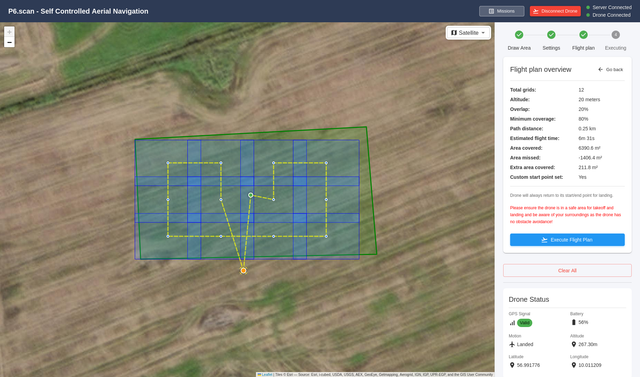
\includegraphics[width=0.95\textwidth]{7. Figures/Frontend/frontend-overview.png}
    \caption{Overview of the main SCAN frontend interface, showing the interactive map, control panel, and status indicators.}
    \label{fig:frontend-overview}
\end{figure}

The main interface is divided into two primary sections: the interactive map area on the left and the control and information panel on the right (see Figure~\ref{fig:frontend-overview}). This split layout allows users to interact with the mission area while simultaneously adjusting settings, monitoring status, and viewing logs.

At the top of the interface, a persistent header bar displays the system title, connection status indicators for both the server and drone, and quick access buttons for switching between the main mission interface and the missions archive. The status indicators use color-coded pulsing icons and concise labels to provide immediate feedback on connectivity.

The central map component enables users to define the search area by drawing polygons, set custom start points, and visualize the planned flight path and waypoints. The map supports both satellite and street views, and overlays real-time drone position and flight progress. Contextual instructions and controls appear above the map to guide the user through each step.

On the right, the control and information panel contains a stepper that visually tracks the user's progress through the mission setup stages: drawing the area, adjusting settings, and executing the flight. Below the stepper, users can configure flight parameters such as altitude, overlap, and coverage, with integrated tooltips for each input to provide guidance. The panel also includes buttons for grid calculation and flight execution, displays the latest captured image, provides a detailed drone status summary, and features a live terminal log of system events and flight actions. The log section can be toggled to fullscreen for in-depth review (Refer to Figures ~\ref{fig:frontend-controls}, ~\ref{fig:frontend-log}).


In addition to the main mission workflow, the frontend provides a dedicated Missions page for reviewing completed missions. This page is accessible via the header and presents a list of all stored missions, each displayed as a card with a timestamp and summary (see Figure~\ref{fig:frontend-missions}). Selecting a mission opens a detailed view that includes a gallery of all images captured during the mission, a chronological flight log, and a static map visualizing the mission path, waypoints, and start/end points.

\begin{figure}[H]
    \centering
    \includegraphics[width=0.95\textwidth]{7. Figures/Frontend/frontend-missions.png}
    \caption{The Missions page, listing completed missions for review and analysis.}
    \label{fig:frontend-missions}
\end{figure}

\begin{figure}[H]
    \centering
    \includegraphics[width=0.95\textwidth]{7. Figures/Frontend/frontend-mission-details.png}
    \caption{Detailed mission view, showing captured images, flight log, and mission path.}
    \label{fig:frontend-mission-details}
\end{figure}

\textbf{Component Overview:}
\begin{itemize}
    \item \textbf{Header:} Displays system title, connection status, and navigation.
    \item \textbf{MapComponent:} Handles map rendering, area drawing, waypoint visualization, and real-time drone tracking.
    \item \textbf{ControlsAndInfo:} Contains the stepper, settings form, flight progress, latest image, drone status, and terminal log.
    \item \textbf{MissionsFolder and SelectedMission:} Manage the missions archive, mission selection, and detailed mission review.
    \item \textbf{MissionMap:} Renders the static mission path for completed missions.
    \item \textbf{DroneStatusPanel, TerminalLogs, and supporting controls:} Provide real-time feedback and system transparency.
\end{itemize}

Throughout the interface, contextual instructions, tooltips, and visual highlights guide the user through each step of the workflow. The stepper and dynamic instructions ensure that users always know what to do next, while real-time updates and logs keep them informed of system status and mission progress.

This structured and modular approach ensures that the SCAN frontend remains intuitive, informative, and robust, supporting efficient mission planning, execution, and review for all users.

\subsection{Intuitive Interactions}
\label{sec:intuitive-interactions}
A core objective of the SCAN frontend is to provide an interface that feels immediately understandable and easy to use, even for users with minimal prior experience. 
This is achieved by applying established principles from cognitive psychology and user interface (UI) design, ensuring that the interface not only looks modern but also aligns with how users naturally perceive and interact with digital systems.

\subsubsection{Step-by-Step Guidance and Progressive Disclosure}

The mission workflow is structured as a clear sequence of stages, visually represented by a stepper component in the control panel (see Figure~\ref{fig:frontend-controls}). 
This design leverages \textbf{Hick’s Law}, which states that the time required to make a decision increases with the number and complexity of choices presented~\cite{hickslaw}. 
By breaking the mission process into discrete, labeled steps (e.g., Draw Area, Settings, Flight Plan, Executing), the interface reduces cognitive load and decision fatigue, making complex tasks approachable for all users~\cite{hickslaw}. 
Progressive disclosure is further employed: only the most relevant controls and information are shown at each stage, while additional options and explanations are revealed contextually, such as through tooltips and overlays.

\subsubsection{Gestalt Principles for Visual Clarity}

The layout and grouping of interface elements are informed by several \textbf{Gestalt principles}~\cite{gestalt_ui}:
\begin{itemize}
    \item \textbf{Proximity:} Related controls (such as input fields for flight parameters) are placed close together, making their relationship immediately apparent.
    \item \textbf{Common Region:} Visual boundaries, such as cards or panels, group related information (e.g., drone status, terminal logs), reinforcing their functional association.
    \item \textbf{Similarity:} Interactive elements (like buttons and icons) use consistent colors and shapes, helping users quickly identify actionable items.
    \item \textbf{Continuity:} The arrangement of steps and the visual flow of the map drawing process guide the user's eye naturally from one action to the next.
\end{itemize}
These principles are visible throughout the interface, for example in the grouping of settings fields and the visual highlighting of the current workflow step (see Figure~\ref{fig:frontend-controls} and Figure~\ref{fig:frontend-tooltips}).

\subsubsection{Immediate Visual Feedback and Error Prevention}

User actions are met with instant visual feedback. When drawing a mission area on the map, vertices and edges are highlighted in real time, and contextual instructions above the map guide the user (see Figure~\ref{fig:frontend-map}). 
Progress indicators, confirmation dialogs, and color-coded status messages keep users informed of system state and prevent errors before they occur. 
For instance, critical actions such as starting a mission require explicit confirmation, while potentially destructive actions (like clearing a drawn area) are disabled unless applicable. 
This approach follows best practices for error prevention and user control in interactive systems~\cite{ui_principles}.

\subsubsection{Direct Manipulation and Fitts’s Law}

Interactive elements such as map markers, resizable panels, and drag-and-drop dividers are sized and positioned to maximize usability, in accordance with \textbf{Fitts’s Law}~\cite{fitts_ui}. 
Larger targets and minimized distances between related controls reduce the effort required for precise actions, making the interface feel responsive and efficient. 
For example, the start point marker on the map is easily draggable, and the terminal log can be resized intuitively by dragging a clearly indicated divider (see Figure~\ref{fig:frontend-map} and Figure~\ref{fig:frontend-log}).

\subsubsection{Summary of Intuitive Design}

By grounding the SCAN frontend in academic UI design principles---including Gestalt laws, Hick’s Law, and Fitts’s Law---the system ensures that users are guided, informed, and protected from errors at every stage. 
The result is an interface that feels natural, reduces training time, and supports both novice and expert users in accomplishing complex drone missions with confidence.

\begin{figure}[H]
    \centering
    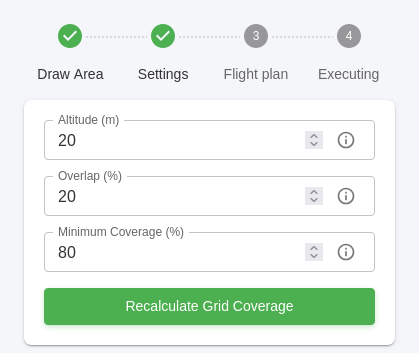
\includegraphics[width=0.95\textwidth]{7. Figures/Frontend/frontend-controls.png}
    \caption{The control and information panel, showing the stepper navigation and grouped settings. The current workflow step is visually highlighted, and related controls are grouped by proximity and common region.}
    \label{fig:frontend-controls}
\end{figure}

\begin{figure}[H]
    \centering
    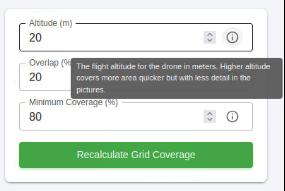
\includegraphics[width=0.95\textwidth]{7. Figures/Frontend/frontend-tooltips.png}
    \caption{Settings form with contextual tooltips. Progressive disclosure and similarity principles help users understand each parameter without overwhelming the interface.}
    \label{fig:frontend-tooltips}
\end{figure}

\begin{figure}[H]
    \centering
    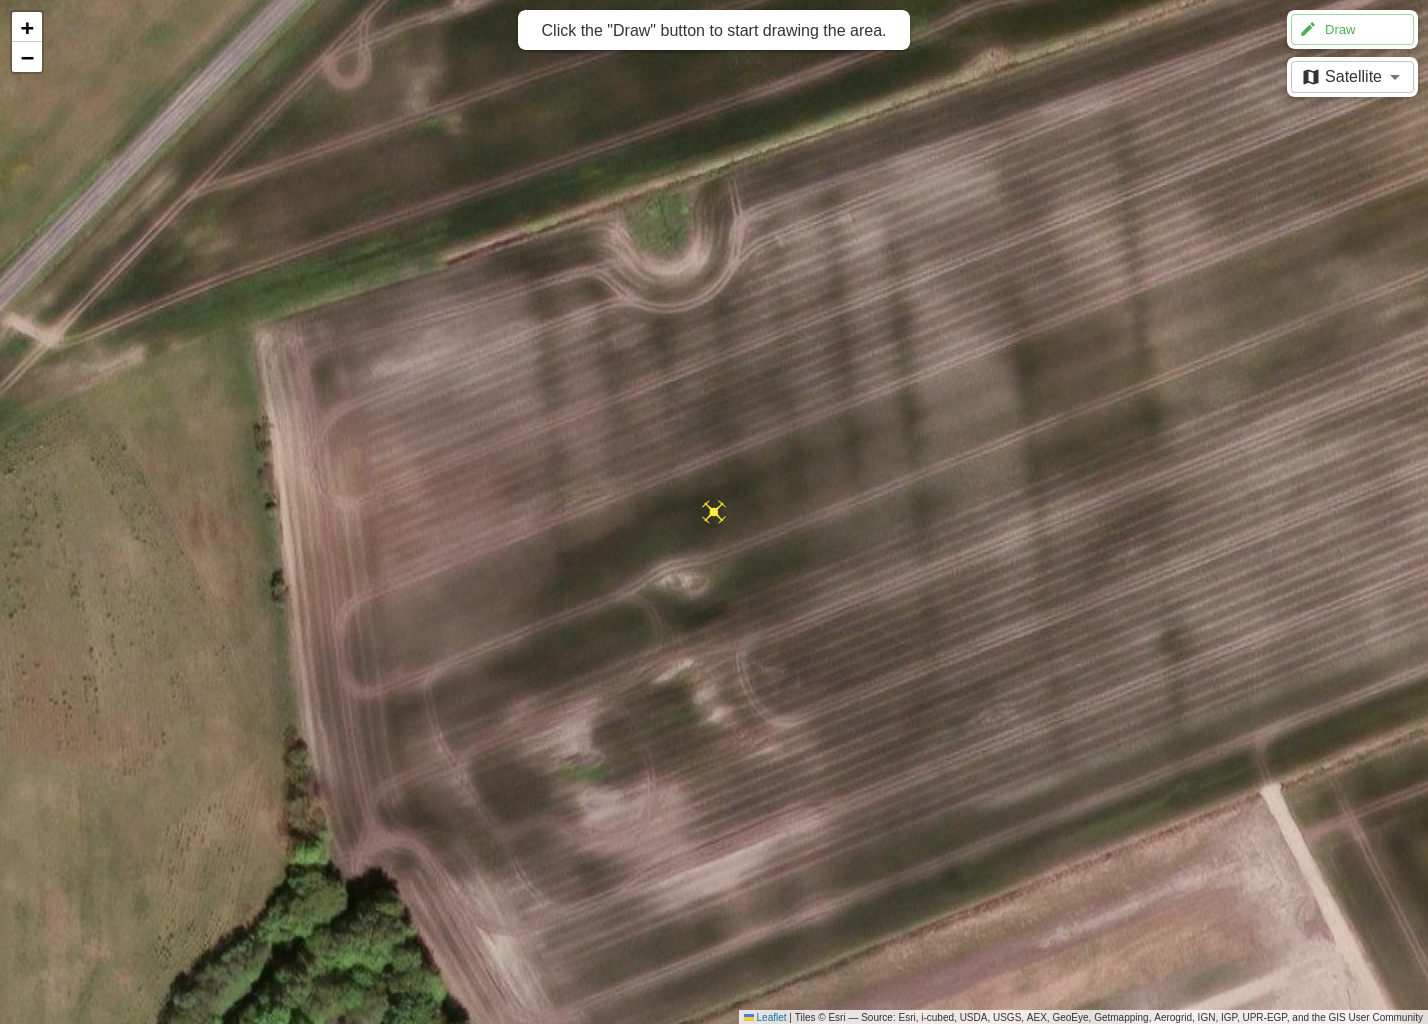
\includegraphics[width=0.95\textwidth]{7. Figures/Frontend/frontend-map-1.png}
    \caption{Map drawing mode, showing real-time feedback as the user defines the mission area. Visual highlights and continuity guide the user through the polygon drawing process.}
    \label{fig:frontend-map-draw}
\end{figure}

\begin{figure}[H]
    \centering
    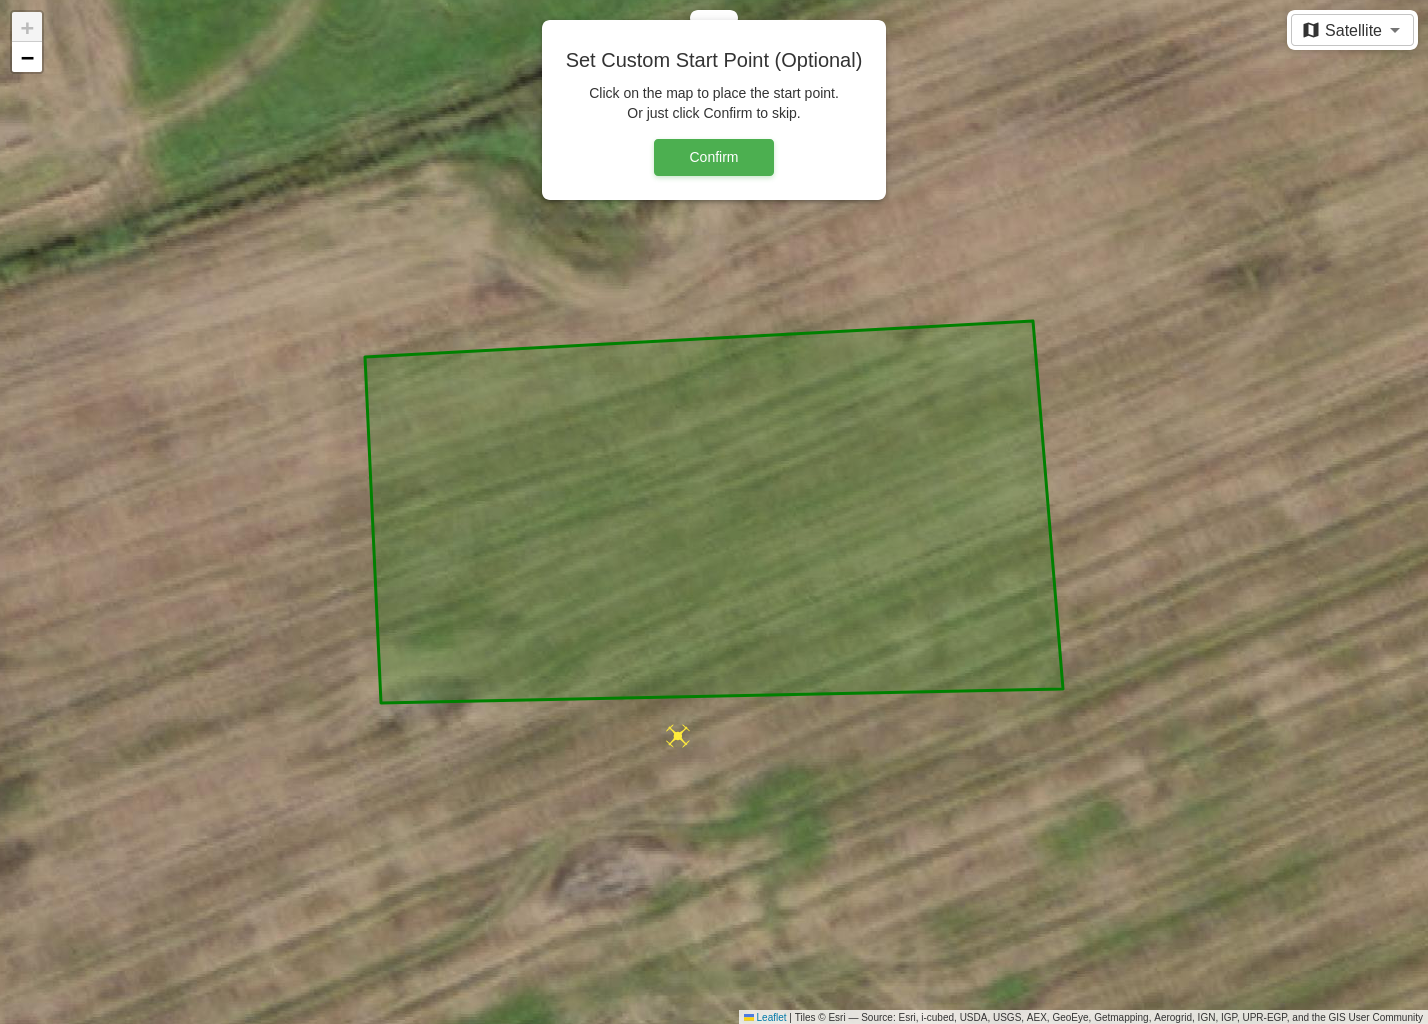
\includegraphics[width=0.95\textwidth]{7. Figures/Frontend/frontend-map-2.png}
    \caption{Selecting the custom start point after area definition. The interface provides clear instructions and visual cues to guide the user through start point selection.}
    \label{fig:frontend-map-setstart}
\end{figure}

\begin{figure}[H]
    \centering
    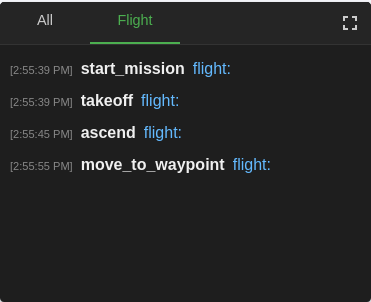
\includegraphics[width=0.95\textwidth]{7. Figures/Frontend/frontend-log.png}
    \caption{Terminal log with drag-to-resize divider. Interactive elements are sized and positioned for ease of use, following Fitts’s Law.}
    \label{fig:frontend-log}
\end{figure}
    
    % Academic references for laws and principles
    \begin{thebibliography}{9}
    \bibitem{hickslaw}
    W. E. Hick, ``On the rate of gain of information,'' \emph{Quarterly Journal of Experimental Psychology}, vol. 4, no. 1, pp. 11–26, 1952.
    
    \bibitem{gestalt_ui}
    S. Palmer, \emph{Vision Science: Photons to Phenomenology}, MIT Press, 1999.
    
    \bibitem{fitts_ui}
    P. M. Fitts, ``The information capacity of the human motor system in controlling the amplitude of movement,'' \emph{Journal of Experimental Psychology}, vol. 47, no. 6, pp. 381–391, 1954.
    
    \bibitem{ui_principles}
    J. Nielsen, ``10 Usability Heuristics for User Interface Design,'' Nielsen Norman Group, 1994.
    
    \end{thebibliography}
    
    Note: If you wish to use your own bibliography management, you can remove or adapt the bibliography block. Update figure filenames as needed to match your project. All academic principles referenced are supported by the search results and are standard in the UI/UX literature.

\subsection{Real-Time Data Visualization}
\label{sec:realtime-visualization}

A central feature of the SCAN frontend is its ability to visualize live data streams from the drone and backend system, ensuring users receive immediate feedback and maintain full situational awareness throughout each mission. 
This is accomplished by leveraging WebSockets for persistent, low-latency communication between the backend (Python) and frontend (ReactJS), enabling the interface to update instantly as new information arrives.

\subsubsection{Live Telemetry and Map Updates}
As soon as the drone’s position, altitude, or battery status changes, the backend emits telemetry events via Socket.IO. 
The frontend listens for these updates and immediately reflects them on the interactive map and in the status panel. 
The drone’s current position and recent trajectory are visualized in real time, allowing users to monitor mission progress and respond quickly to any unexpected behavior (see Figure~\ref{fig:frontend-overview}).

\subsubsection{Instant Flight Logs}
All significant system events---such as takeoff, waypoint completion, photo capture, and error notifications---are streamed from the backend as log messages. 
These logs appear instantly in the terminal log panel, with color coding and timestamps to help users quickly identify warnings or issues (see Figure~\ref{fig:frontend-log}). 
This transparency is crucial for building user trust and supporting rapid troubleshooting during live operations.

\subsubsection{Real-Time Image and Detection Results}
Whenever the drone captures and processes a new image, the backend immediately sends the image data and detection results to the frontend. 
The latest image is displayed in the control panel, with a visual indicator showing whether the detection was successful. 
This immediate feedback confirms camera operation and object detection performance, reducing uncertainty and supporting mission objectives.

\subsubsection{User Confidence and Situational Awareness}
By ensuring that all telemetry, logs, and images are updated in real time, the SCAN frontend provides users with a continuous, accurate picture of the drone’s status and mission progress. 
The use of WebSockets eliminates the delays associated with traditional polling, resulting in a responsive interface that supports confident and informed decision-making throughout the mission lifecycle~\cite{syncfusion_ws}.

\subsection{Accessibility and Responsiveness}
\label{sec:accessibility-responsiveness}

The SCAN frontend is designed to remain usable and visually coherent across a wide range of devices and screen sizes. The Material UI foundation, mentioned in Section 4.1, provides a responsive grid system and adaptive layouts that automatically adjust to desktops, laptops, and tablets. The split layout, which separates the interactive map from the control panel, remains functional and clear even when the window is resized or when users zoom in using browser or operating system scaling features. All interface components scale proportionally, ensuring that no part of the layout breaks or becomes inaccessible under different viewing conditions.

Basic accessibility is supported through Material UI’s default behaviors. Most form elements have appropriate labels and can be navigated using the keyboard, while focus outlines are visible for standard controls. Color contrast and text sizing are generally reasonable by default, and users with visual impairments can benefit from the interface’s ability to scale without loss of functionality. However, no custom enhancements for keyboard navigation or screen reader support have been implemented, and accessibility beyond the defaults provided by Material UI has not been explicitly addressed.

In summary, the frontend offers robust responsiveness and a baseline level of accessibility. Further improvements could be made by introducing explicit accessibility testing, increasing color contrast where necessary, and enhancing support for keyboard navigation and alternative input methods.

\subsection{Reliability and Error Handling}
\label{sec:reliability-error-handling}

The SCAN frontend is designed to maintain reliability and support safe operation, even when facing connection issues, invalid user input, or unexpected errors. While Section 4.3 discusses visual feedback from a user interaction perspective, this section focuses on the technical mechanisms that ensure system reliability and error management.

\subsubsection{Connection Handling}
A persistent header at the top of the interface displays the status of the backend server and drone connections using clear, color-coded indicators. If either connection is lost, the interface displays an overlay message and disables map interactions and controls until the connection is restored. The frontend automatically attempts to reconnect to the backend and notifies users of reconnection attempts and status changes, helping to reduce confusion during temporary outages.

\subsubsection{Input Validation and User Actions}
All flight parameter forms, such as those for altitude (restricted to 0--40 meters) and coverage (0--100\%), use built-in validation to prevent invalid inputs. Action buttons like ``Confirm,'' ``Draw,'' and ``Execute Flight'' are disabled unless the current state and inputs are valid and safe. Contextual tooltips and instructions help guide users to correct any mistakes before proceeding. For critical actions, such as starting a mission or clearing the drawn area, explicit confirmation dialogs are shown to prevent accidental operations.

\subsubsection{Unexpected Errors and Feedback}
If an unexpected error occurs in the frontend, the application is designed to handle it gracefully without crashing the entire interface. Errors and warnings received from the backend are displayed in real time in the terminal log panel, using color coding to indicate severity. This transparency allows users to review issues and understand the system's state at any time.

\subsubsection{User Feedback and Control}
Visual cues such as overlays, disabled buttons, and clear status messages ensure that users are always aware of the current system state. Where appropriate, users can cancel or reset actions, and the interface prevents operations that could lead to undefined or unsafe situations.

Overall, the SCAN frontend prioritizes reliability by proactively handling connection problems, invalid inputs, and unexpected errors. These mechanisms keep users informed, prevent mistakes, and ensure safe, confident operation throughout the mission workflow.

\section{Data Management}
% How you store and organize photos, logs, and mission data.

\section{Implementation Challenges}
% Any major challenges faced during implementation and how you solved them.

\section{Summary}
% Short summary of the implementation and transition to the next chapter.
\chapter{Testing}

The testing approach for this project covers five main types of tests: \textbf{unit tests}, \textbf{integration tests}, \textbf{system tests}, \textbf{usability tests}, and \textbf{acceptance tests}. Unit tests, integration tests, and system tests are primarily conducted to ensure reliability: unit tests check individual components in isolation, integration tests verify the interaction between modules, and system tests assess the complete system in a simulated or controlled environment. Usability tests evaluate how intuitive and user-friendly the interface is for operators. Acceptance tests confirm that the final product meets the specified requirements and functions correctly in real-world conditions.

All test cases follow the \textbf{AAA (Arrange-Act-Assert)} pattern to ensure a consistent and structured testing process, with usability tests following a task-based assessment methodology with user feedback collection.

\section{Unit Testing}
\section{Integration Testing}
\section{System Testing}
\section{Acceptance Testing}

The acceptance test for the SCAN system is designed to validate the complete workflow in a realistic search and rescue scenario. The test was carried out on a beach in Hals, Denmark.

\subsection{Test Procedure}

\begin{enumerate}
    \item \textbf{Site Preparation:} The team set up the drone and the SCAN system on a laptop at the beach (see Figure~\ref{fig:acceptance-test-setup}).
    \item \textbf{Test Subject Placement:} One group member positioned themselves in the water to simulate a person in distress (see Figure~\ref{fig:test-subject-placement}).
    \item \textbf{Flight Execution:} The drone was launched and flew at an altitude of 20 meters, following a predefined search pattern over the water.
    \item \textbf{Detection:} The onboard camera captured images, which were processed by the YOLO-based detection model running on the laptop.
    \item \textbf{Landing:} After completing the search pattern, the drone autonomously returned and landed at its starting position.
    \item \textbf{Result Evaluation:} The test was considered successful if the drone followed the planned route, landed at the starting position, and the YOLO model correctly detected the group member in the water.
\end{enumerate}

\subsection{Success Criteria}

\begin{itemize}
    \item The drone autonomously follows the generated flight path at the specified altitude.
    \item The drone lands at its original starting position after completing the mission.
    \item The YOLO detection model identifies the group member in the water and marks their position in the system interface.
\end{itemize}

\subsection{Documentation}

Photographic documentation is included, showing the testing site and the group member in the water, to support the acceptance test results.

\begin{figure}[H]
    \centering
    \includegraphics[width=0.8\textwidth]{7. Figures/acceptance-test-setup.jpg}
    \caption{Acceptance test setup at the beach in Hals, Denmark}
    \label{fig:acceptance-test-setup}
\end{figure}

\begin{figure}[H]
    \centering
    \includegraphics[width=0.8\textwidth]{7. Figures/test-subject-placement.jpg}
    \caption{Test subject placement: group member in the water}
    \label{fig:test-subject-placement}
\end{figure}

\begin{figure}[H]
    \centering
    \includegraphics[width=0.8\textwidth]{7. Figures/detection-result.jpg}
    \caption{Detection result: YOLO model identifies the group member in the water}
    \label{fig:detection-result}
\end{figure}

\subsection{Result}

As shown in Figure~\ref{fig:detection-result}, the acceptance test was successful. The drone autonomously followed the planned route, landed at its original starting position, and the YOLO detection model correctly identified the group member in the water. This demonstrates that the SCAN system meets its intended requirements and is capable of supporting search and rescue operations in real-world conditions.
\chapter{Discussion}

This chapter reviews the development process of the Self-Controlled Aerial Navigation (SCAN) project. It describes how the plan-driven, waterfall methodology was applied, and discusses the main decisions made during each project phase. The chapter also covers challenges faced, reasons for key choices, and areas where the process could have been improved. In addition, it includes a risk analysis and suggestions for future work, providing guidance for teams who may continue developing the SCAN project.

\section{Methodology}

This section outlines the methodological approahc employed in the development of the Self-Controlled Aerial Navigation (SCAN) project. The methodology consists of project management techniques, version control strategies, an the utilization of various tools to ensure a structured development process.

\subsection{Project Management}
The project management approach for SCAN is centered around the use of GitHub Projects, an integrated tool within the GitHub platform. This tool provides different kinds of features to organise and keep track of project development.

\subsubsection{Kanban Board}
A Kanban board as shown in figure \ref{fig:kanban-board} is implemented using GitHub Projects to visualize and manage the workflow of tasks throughout the project lifecycle. 

The board is structured into five columns:

\begin{itemize}
    \item Roadmap: Contains high-level project milestones and objectives.
    \item Docs Todo: Lists documentation tasks that need to be completed.
    \item System Todo: Consists of pending system development tasks.
    \item In Progress: Shows tasks currently being worked on.
    \item Done: Contains completed tasks.
\end{itemize}

\FloatBarrier

\begin{figure}
    \centering
    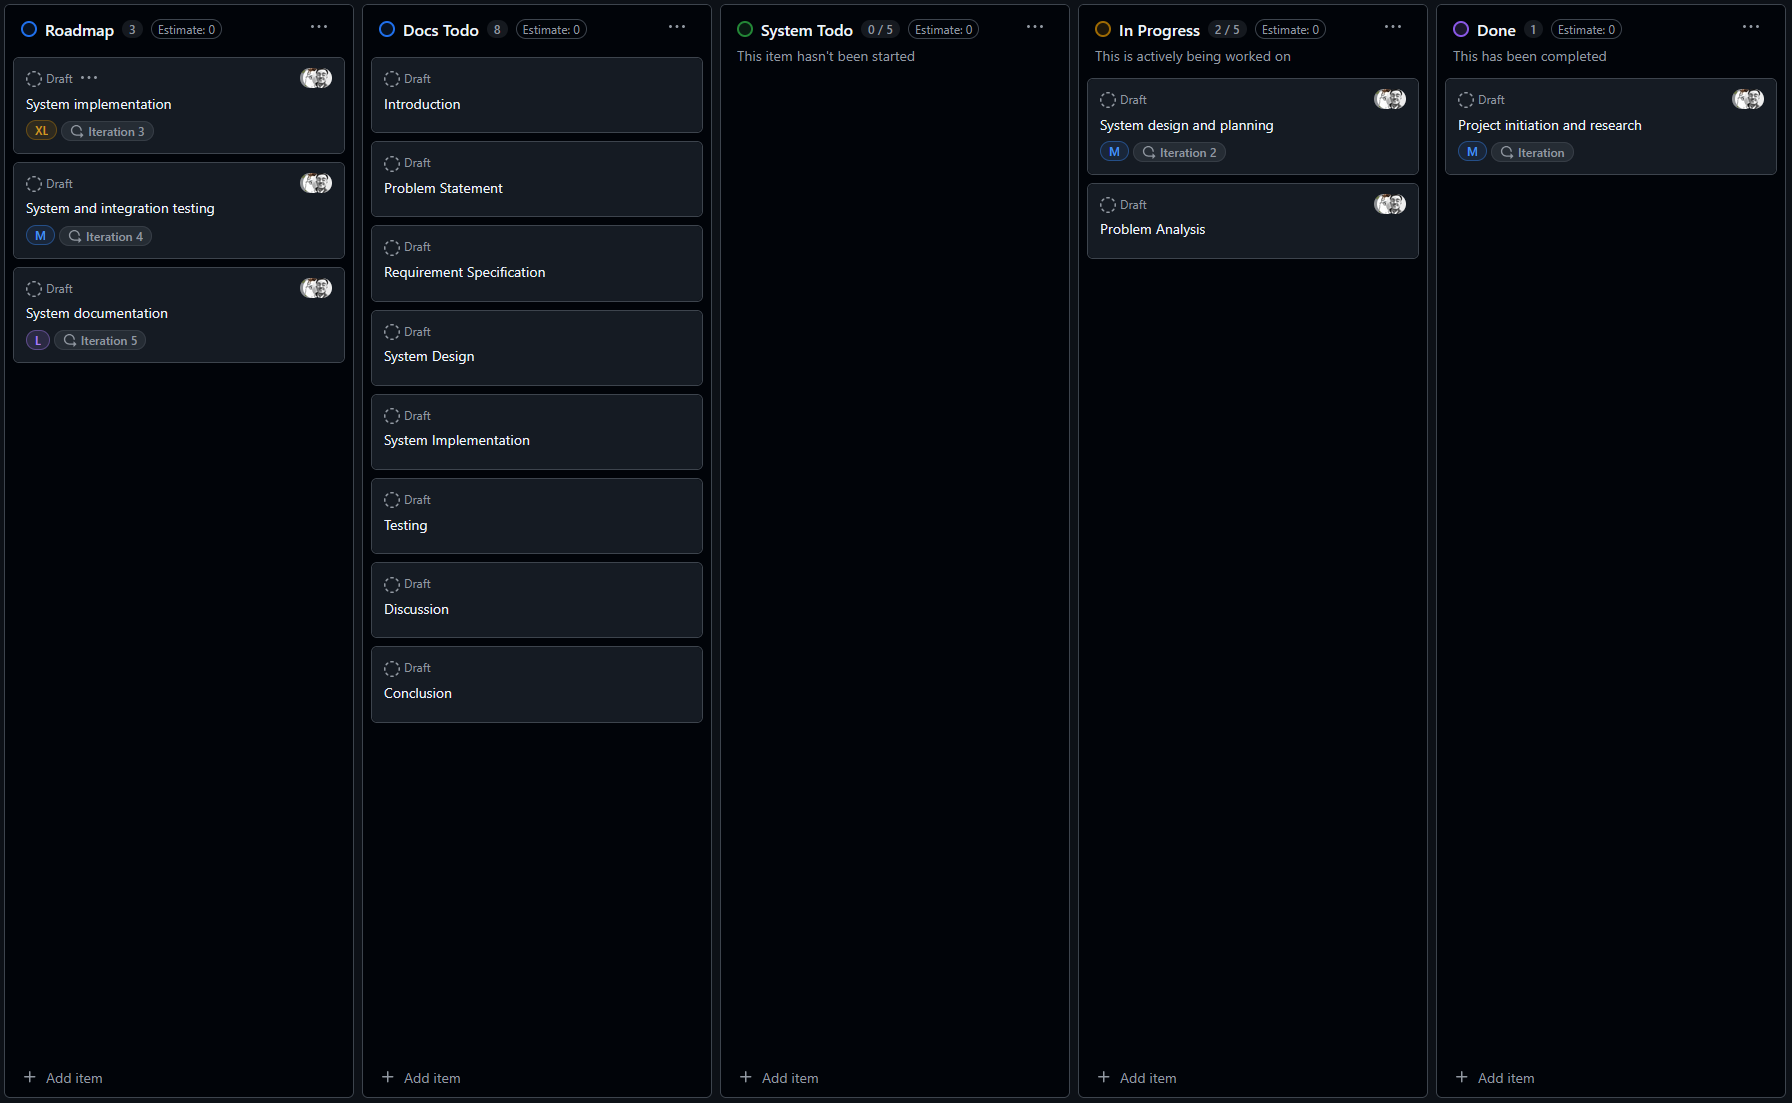
\includegraphics[width=1\linewidth]{7. Figures/Methodology/Kanbanboard.png}
    \caption{Kanban board utilized in the project}
    \label{fig:kanban-board}
\end{figure}

\subsubsection{Project Roadmap}

In addition to the Kanban board, a project roadmap is utilized to provide a timeline view of major project phases. The roadmap is divided into five phases:

\begin{enumerate}
    \item Project Initiation and Research (09/02/2025 - 21/02/2025).
    \item System Design and Planning (24/02/2025 - 07/03/2025).
    \item System Implementation (10/03/2025 - 02/05/2025).
    \item System and Integration Testing (05/05/2025 - 11/05/2025).
    \item System Documentation (12/05/2025 - 28/05/2025).
\end{enumerate}

Each phase is further broken down into specific tasks and objectives. For instance, the Project Initiation and Research phase includes:

\begin{itemize}
    \item Defining the initial project scope and objectives.
    \item Conducting literature review on drone navigation and control.
    \item Analyzing existing solutions and technologies.
    \item Drafting initial problem statement.
\end{itemize}

Similarly, the System Design and Planning phase consists of:

\begin{itemize}
    \item Refining problem statement and research questions.
    \item Developing the system architecture.
    \item Finalizing the report structure.
    \item Beginning initial report writing (problem analysis, statement, etc.).
\end{itemize}

This roadmap serves as a high-level guide for the project time, allowing for better resource allocation and also progress tracking. It should be noted however, that the project is not following the waterfall model but instead a more iterative model allowing for adjustments throughout the process and more flexibility. 

\subsection{Version Control}
Version control is an important aspect of the development process to ensure code integrity and provide collaboration among the team members. For the SCAN project, Git is employed as the version control system, with GitHub serving as the remote repository host.

\subsubsection{Branching Strategy}
A feature-based branching strategy is adopted for the project. The main branch serves as the stable, production-ready codebase, while the dev-main branch serves as the stage or development-level codebase. For each new feature or significant change, a new branch is created from the dev-main branch. After completion of a branch, it is merged into the dev-main branch and after finalizing a development stage, the dev-main development branch is merged into the main production branch.

The branching workflow is as follows:
\begin{enumerate}
    \item Create a new branch for a feature or bug fix from the dev-main branch.
    \item Develop and test the feature in isolation.
    \item Create a pull request for code review.
    \item After CI checks and approval, merge the feature branch back into the dev-main branch.
    \item Delete the feature branch after successful merge.
\end{enumerate}

\subsection{Continuous Integration (CI)}

While Continuous Integration (CI) is implemented in the SCAN project, Continuous Deployment (CD) is not deemed necessary due to the specific operational characteristics of the drone system. The reasons for this decision are as following.

\begin{enumerate}
    \item Local Execution Environment: The SCAN system is designed to operate with the backend running locally on a machine that directly interfaces with the drone or by uploading the final backend output directly into the drone for a disconnected autonomous operation. This local execution model differs significantly from typical web or cloud-based applications where CD is more commonly used.
    \item Autonomous Drone operation: The primary goal of the SCAN system is to enable autonomous drone navigation. Once the flight plan and navigation algorithms are loaded onto the drone, it is designed to operate independently without constant connection to an external system. As a fallback, the only connection to the drone would be between the backend and the drone itself, which would require the backend to be within range of the drone.
\end{enumerate}

GitHub Actions is utilized to set up CI workflows. These workflows are triggered on every push to the repository and on the creation of pull requests. The CI process includes the following steps:

\begin{enumerate}
    \item Code compilation: Ensures that the code builds successfully.
    \item Unit testing: Runs the project's unit tests to verify individual components.
    \item Integration testing: Performs tests on integrated components to verify behavior of multiple integrated components.
\end{enumerate}

If any of these steps fail, the CI process is halted, and the team members are notified of the failure. 

\subsection{Communication and Collaboration}
Communication and collaboration are very important for the success of the SCAN project. The following practices are implemented to ensure this:

\begin{itemize}
    \item Team meetings: Project development 4 times a week (mostly) with informal meetings of project progress and upcoming tasks.
    \item Discord: Used for real-time communication and quick discussions.
    \item GitHub discussions: Issue descriptions and comments are perhaps going to be utilized for longer, asynchronous conversations about project direction and technical decisions.
    \item Shared documentation: Notion with a project-focused directory for project-relevant information.
\end{itemize}

\section{What could we have done different?}

\subsection{Potential Improvements Through Early Risk Analysis}

A structured risk analysis at the start of the project could have prevented several avoidable issues. One of the main problems was the immediate reliance on the actual drone for testing. The project had access to a simulation tool designed for safe and controlled testing of navigation and control algorithms. However, the simulation tool was not set up or used until after the drone had already been damaged during early physical tests.

If the simulation tool had been configured and integrated into the workflow from the beginning, initial development and testing could have taken place in a virtual environment. This would have reduced the risk of hardware damage and allowed for faster iterations without the delays caused by repairing or replacing physical equipment. The lack of early simulation testing resulted in unnecessary downtime when the only available drone was damaged, which could have been avoided.

An early risk analysis would likely have identified the risks associated with hardware dependency and highlighted the benefits of simulation-based testing. This approach would have allowed the team to validate core functionalities and catch errors in a safe environment before moving to real-world tests. For future projects, setting up and prioritizing the use of simulation tools at the start is recommended, as it minimizes the risk of equipment failure and project delays.

\section{Future Work}

\subsection{The Advantages of Thermal Cameras for Drone-Based Water Rescue}

The current drone-based water rescue solution utilizes standard RGB cameras and a YOLOv8 model to detect humans in open water. While effective during daylight and clear weather, this approach has reliability limitations in challenging conditions. Integrating thermal cameras would address these limitations and improve performance.

\subsubsection{Enhanced Reliability with Thermal Imaging}

Thermal cameras detect heat signatures rather than visible light, offering key advantages:

\begin{itemize}
    \item \textbf{Operation in Low-Light and Night Conditions:} Standard cameras fail after sunset, while thermal cameras enable 24/7 operation\cite{advexure_thermal_sar}.
    \item \textbf{Performance in Adverse Weather:} Thermal imaging penetrates fog and ignores water surface glare, maintaining detection capability during rain or poor visibility.
    \item \textbf{Faster Detection:} Heat signatures simplify human identification for AI models, reducing missed detections from camouflage or shadows.
\end{itemize}

\subsubsection{Combining Camera Technologies for Optimal Results}

For the most effective search and rescue operations, especially in varied lighting and weather conditions, combining multiple camera types is recommended:

\begin{itemize}
    \item \textbf{Daytime Operations:} Using both RGB cameras and thermal cameras allows for cross-verification, improving detection accuracy. RGB cameras provide high-resolution visual information, while thermal cameras highlight heat signatures that might be missed in cluttered visual backgrounds.
    \item \textbf{Nighttime Operations:} A combination of thermal cameras and night vision cameras is ideal. Thermal cameras detect heat signatures in complete darkness, while night vision cameras amplify available light, providing additional visual context and helping to identify objects or obstacles that may not emit heat.
\end{itemize}

This multi-sensor approach increases the chances of detecting persons in the water under all conditions and reduces the likelihood of false negatives.

\subsubsection{Limitations and Cost Considerations}

\begin{itemize}
    \item \textbf{High Equipment Costs:} Thermal drones range from \$6,500 to \$24,000+ versus standard camera drones\cite{dslrpros_sar_drones}.
    \item \textbf{Environmental Constraints:} Reduced effectiveness when body and water temperatures are similar (e.g., after prolonged cold immersion). Thermal cameras cannot see through water, limiting detection if a person is submerged\cite{fireapparatus_thermal_water_rescue}. Combining thermal cameras with RGB or night vision cameras can help mitigate these limitations by providing additional visual information when thermal contrast is low or when a person is partially submerged.
    \item \textbf{Regulatory Challenges:} Additional restrictions may apply for nighttime or over-water operations.
\end{itemize}

\subsubsection{Comparative Summary}

\begin{table}[h]
\centering
\begin{tabular}{|l|l|l|l|}
\hline
\textbf{Feature} & \textbf{RGB Camera} & \textbf{Night Vision} & \textbf{Thermal Camera} \\ \hline
Daytime Operation & Yes & No & Yes \\ \hline
Nighttime Operation & No & Yes & Yes \\ \hline
Fog/Glare Performance & Limited & Limited & Excellent \\ \hline
Detection Reliability & Moderate & Moderate & High \\ \hline
Cost & Lower & Moderate & Higher \\ \hline
\end{tabular}
\caption{Comparison of camera systems for water rescue drones}
\end{table}

\subsubsection{Conclusion}

Thermal cameras substantially improve reliability for water rescue drones by enabling 24/7 operation and performance in adverse weather. Combining thermal imaging with RGB cameras during the day, and with night vision cameras during the night, provides the most robust solution for detecting persons in the water. While cost and regulatory factors require consideration, the life-saving potential and improved consistency make a multi-sensor approach the preferred choice for critical search and rescue missions.




\subsection{Multi-Drone Support}

While multi-drone functionality was not fully implemented in the current project iteration, preliminary exploration demonstrated its potential to significantly improve mission efficiency. A custom Python script was developed to simulate multi-drone operation by dividing search areas into segments, with each drone assigned a specific zone using proximity-based allocation. This section outlines the technical foundations and benefits observed during simulation.

\textbf{Key Technical Advantages}
\begin{enumerate}
    \item \textbf{Parallel Coverage:}
    \begin{itemize}
        \item Single-drone systems require sequential scanning of entire search grids.
        \item Multi-drone implementations split grids into non-overlapping segments (see Figure\ref{fig:multi_drone}), enabling simultaneous coverage.
        \item Simulation results showed a near-linear reduction in mission duration with each added drone (e.g., 2 drones $\approx$ 50\% time reduction).
    \end{itemize}
    \item \textbf{Proximity-Based Assignment:}
    \begin{itemize}
        \item Drones are assigned grid segments closest to their predefined start points.
        \item This minimizes initial travel distance compared to centralized allocation methods.
    \end{itemize}
    \item \textbf{Collision Avoidance:}
    \begin{itemize}
        \item Exclusive grid assignments eliminate mid-air collision risks during missions.
    \end{itemize}
    \item \textbf{Scalable Architecture:}
    \begin{itemize}
        \item The core path planning algorithm remained unchanged in simulations.
        \item New drones only require segment assignment logic and start point coordinates.
    \end{itemize}
\end{enumerate}

\textbf{Search \& Rescue Implications}

For aquatic person detection scenarios, multi-drone deployment could:
\begin{itemize}
    \item Reduce critical response times in time-sensitive emergencies
    \item Enable coverage of larger search areas without sacrificing resolution
    \item Provide redundancy if individual drones malfunction
\end{itemize}

\textbf{Implementation Challenges}

The simulation revealed two key requirements for practical implementation:
\begin{enumerate}
    \item \textbf{Centralized Coordination:} A master system to allocate grid segments and monitor drone statuses.
    \item \textbf{Hardware Standardization:} Identical drone specs for consistent flight performance and camera capabilities.
\end{enumerate}

While full integration remains future work, the simulation (see Figure\ref{fig:multi_drone}) validated the core technical approach. Implementing multi-drone support would require additional development in fleet coordination interfaces and real-time status monitoring, but the foundational path planning architecture appears directly adaptable.

\begin{figure}[h]
    \centering
    \includegraphics[width=0.8\textwidth]{multi_drone_simulation}
    \caption{Simulation output showing three drones covering partitioned grid segments using proximity-based assignment}
    \label{fig:multi_drone}
\end{figure}

\chapter{Conclusion}

\bibliographystyle{plain}
\bibliography{Bibliography}


\end{document}